\documentclass[11pt]{article}

% Change "review" to "final" to generate the final (sometimes called camera-ready) version.
% Change to "preprint" to generate a non-anonymous version with page numbers.
\usepackage[final]{acl}

% Standard package includes
\usepackage{times}
\usepackage{latexsym}
\usepackage{booktabs}
\usepackage{pifont}
\usepackage{xcolor,colortbl}
\usepackage{threeparttable}
\usepackage[table]{xcolor}
\usepackage{multirow} 
\usepackage{amsmath}
\usepackage{booktabs} 
\usepackage{soul}

% \sethlcolor{yellow!25}
\sethlcolor{blue!12}

% For proper rendering and hyphenation of words containing Latin characters (including in bib files)
\usepackage[T1]{fontenc}
% For Vietnamese characters
% \usepackage[T5]{fontenc}
% See https://www.latex-project.org/help/documentation/encguide.pdf for other character sets

% This assumes your files are encoded as UTF8
\usepackage[utf8]{inputenc}

% This is not strictly necessary, and may be commented out,
% but it will improve the layout of the manuscript,
% and will typically save some space.
\usepackage{microtype}

% This is also not strictly necessary, and may be commented out.
% However, it will improve the aesthetics of text in
% the typewriter font.
\usepackage{inconsolata}

%Including images in your LaTeX document requires adding
%additional package(s)
\usepackage{graphicx}

\usepackage{xspace}

% If the title and author information does not fit in the area allocated, uncomment the following
%
%\setlength\titlebox{<dim>}
%
% and set <dim> to something 5cm or larger.

\title{From Proof to Program: Characterizing Tool-Induced Reasoning Hallucinations in Large Language Models}

% Author information can be set in various styles:
% For several authors from the same institution:
% \author{Author 1 \and ... \and Author n \\
%         Address line \\ ... \\ Address line}
% if the names do not fit well on one line use
%         Author 1 \\ {\bf Author 2} \\ ... \\ {\bf Author n} \\
% For authors from different institutions:
% \author{Author 1 \\ Address line \\  ... \\ Address line
%         \And  ... \And
%         Author n \\ Address line \\ ... \\ Address line}
% To start a separate ``row'' of authors use \AND, as in
% \author{Author 1 \\ Address line \\  ... \\ Address line
%         \AND
%         Author 2 \\ Address line \\ ... \\ Address line \And
%         Author 3 \\ Address line \\ ... \\ Address line}

% \author{Farima Fatahi Bayat\\
%   Megagon Labs \\
%   \texttt{farima@megagon.ai} \\\And
%   Pouya Pezeshkpour \\
%   Megagon Labs \\
%   \texttt{pouya@megagon.ai} \\\And
%   Estevam Hruschka \\
%   Megagon Labs \\
%   \texttt{estevam@megagon.ai} \\
%   }

\author{
 \textbf{Farima Fatahi Bayat},
 \textbf{Pouya Pezeshkpour},
 \textbf{Estevam Hruschka}
\\
 Megagon Labs
\\
    \{farima, pouya, estevam\}@megagon.ai
\\
}


%\\
%  \textsuperscript{1}Affiliation 1,
%  \textsuperscript{2}Affiliation 2,
%  \textsuperscript{3}Affiliation 3,
%  \textsuperscript{4}Affiliation 4,
%  \textsuperscript{5}Affiliation 5
%\\
%  \small{
%    \textbf{Correspondence:} \href{mailto:email@domain}{email@domain}
%  }
%}
\def \dataset{\textsc{PyMath}\xspace}
\def \task{\textsc{TIM}\xspace}

\newcommand{\farima}[1]{{\color{orange}Farima: #1}}
\newcommand{\pouya}[1]{{\color{violet}Pouya: #1}}
\newcommand{\estevam}[1]{{\color{blue}Estevam: #1}}

\newcommand{\postspace}{\vskip -3mm}
\newcommand{\minipostspace}{\vskip -1mm}

\definecolor{cadmiumgreen}{rgb}{0.0, 0.42, 0.24}
\definecolor{cardinal}{rgb}{0.77, 0.12, 0.23}
\definecolor{cadmiumred}{rgb}{0.89, 0.0, 0.13}
\newcommand*{\promptfont}{\fontfamily{courier}\selectfont}
\usepackage[most]{tcolorbox}
\newtcolorbox[list inside=prompt,auto counter,number within=section]{prompt}[1][]{
    fontupper=\ttfamily\footnotesize,
    boxsep=5pt,
    left=0pt,
    right=0pt,
    top=0pt,
    bottom=0pt,
    boxrule=1pt,
    breakable,
    #1,
}

%%%%%%%%%%%%%%%%%
% \newtcolorbox{minicard}{enhanced, sharp corners, colframe=black!15,
%   colback=white, boxrule=0.3pt, left=4pt, right=4pt, top=4pt, bottom=4pt}


% %
% \usepackage{pifont}
% \newcommand{\good}{\textcolor{green!60!black}{\ding{51}}}
% \newcommand{\bad}{\textcolor{red!70!black}{\ding{55}}}

% \newtcolorbox{logcard}[1]{enhanced, breakable, colback=white, colframe=black!12,
%   title={#1}, colbacktitle=black!3, boxrule=0.4pt}

% %

% \tcbset{colframe=black!10, boxrule=0.4pt, colback=white, coltitle=black, fonttitle=\bfseries}

\newtcolorbox{example}[2][]{%
  enhanced, breakable,
  colback=white,           % white background
  colframe=black!10,
  boxrule=0.4pt,
  coltitle=black,
  fonttitle=\bfseries,
  title={#2},
  #1
}

% \newcommand{\hlb}[1]{\colorbox{yellow!25}{#1}}

% \newcommand{\hlb}[2][blue!12]{
%   \begingroup
%   \setlength{\fboxsep}{2pt}% padding inside the color box
%   \colorbox{#1}{\parbox{\dimexpr\linewidth-2\fboxsep\relax}{#2}}%
%   \endgroup
% }

%%%%%%%%%%%%%%%
\begin{document}
\maketitle
\begin{abstract}

Tool-augmented Language Models (TaLMs) can invoke external tools %estevam, such as code interpreters,
to solve %estevammathematical 
problems beyond their parametric capacity. However, it remains unclear whether these tool-enabled gains reflect trustworthy reasoning.
% Tool-augmented Language Models (TaLMs) extend LMs by incorporating external tools, which enable them to solve complex tasks beyond their parametric knowledge, yet whether these improvements is trustworthy is underexplored. 
% \pouya{the transition is not subtle here, we should first lay the ground first. For example saying using tools result in improvement but we are not sure how and wether the improvement is trsutworthy, so we...} 
Focusing on the Code Interpreter tool,
% \pouya{maybe mention here: focusing on Code Interpreter tool,}
we show that even when tools are selected and executed correctly, TaLMs treat tool outputs as substitutes for reasoning, producing solutions that appear correct but lack coherent justification. We term this failure mode \textbf{T}ool-\textbf{I}nduced \textbf{M}yopia (\textbf{\task{}}), and study it using
% a phenomenon in which access to a tool narrows a model’s reasoning to what the tool can compute, leading to empirical search, premature answer acceptance, or the omission of necessary analytical steps.
\dataset, 
% \estevam{suggestion for the above paragraph: In this work, we show that even when tools are selected and executed correctly, TaLMs frequently treat tool outputs as substitutes for reasoning, producing solutions that appear correct, but lack coherent justification. We term this failure mode \textbf{T}ool-\textbf{I}nduced \textbf{M}yopia (\textbf{\task{}}), and study it focusing on Code Interpreter tool, and evaluate performance on}
a benchmark of 1,679 competition-level mathematical problems for which
% put "from existing datasets" in intro
Python code is \textit{helpful but not sufficient}. We further develop a multi-dimensional evaluation suite to quantify reasoning degradation in TaLMs relative to their non-tool counterparts. Our findings reveal that while TaLMs achieve up to a 19.3 \textit{percentage point} gain in final-answer accuracy, their reasoning behavior consistently deteriorates (e.g., non-tool language models win up to 41.5\% more often in pairwise comparisons of reasoning processes). 
% up to 27.3\% increase in missed logical steps). 
This degradation intensifies with tool use; the more frequently a model invokes tools, the less coherent its reasoning becomes. Moreover, tool use shifts errors from arithmetic mistakes toward global reasoning failures (logic, assumption, creativity).
% ignore for now: ; with \task{} present in \textasciitilde{}55\% of high-risk cases.
% This degradation amplifies with increasing tool use, i.e., the more frequently a model calls tools, the less coherent its reasoning becomes. 
% Moreover, tool use shifts error types toward global reasoning failures (logic/assumption/creativity) while reducing arithmetic mistakes; generated-code complexity shows little correlation with TIM; and a manual audit finds TIM in ~55\% of high-risk cases identified by our evaluation suite.
Finally, we propose a preference-optimization-based framework that realigns TaLMs to use tool outputs as assistive evidence, improving both final-answer accuracy and the reasoning depth under tool use.\footnote{Code and data are available at: \url{https://github.com/megagonlabs/TIM}.}
% Codes and data are available at: \url{https://github.com/megagonlabs/TIM}.
% \pouya{Instead say: We released our dataset and code\footnote{} and create an empty github repo in megagonlabs page (let me know if you need help to do that)}

% Our benchmark, evaluation suite, and mitigation method provide the first comprehensive framework for analyzing and reducing \task{}, paving the way toward more trustworthy tool-augmented reasoning systems. \pouya{you can omit the last line, move it to intro and here just point to the github page and say we make everything public.}
\end{abstract}

\section{Introduction}

Large Language Models (LLMs) have grown increasingly capable, yet relying solely on their parametric knowledge introduces key limitations, including the inability to access real-time or domain-specific information~\citep{yu-ji-2024-information, wang2025actingreasoningmoreteaching}, perform precise computations~\citep{lu-etal-2023-survey}, or fully comprehend user intentions~\citep{qian-etal-2024-tell}. 
To address these shortcomings, Tool-augmented Reasoning (TIR)~\citep{toolformer, gou2024tora} has emerged as a promising paradigm. It enables LLMs to integrate natural language reasoning with external tools. 
% A tool, in this context~\citep{wang2024toolsanywaysurveylanguage}, is a function interface to an external computer program, where the model generates function calls to interact with it. 
% With the advent of TIR, numerous tools, such as web search \citep{asai2024selfrag, 10.5555/3666122.3668004}, 
% document retrieval systems \citep{10.1145/3637528.3671470},
% code interpreters \citep{POTprompting, gao2022pal}, and domain-specific APIs \citep{Qin2023ToolLLMFL}, have augmented the reasoning capabilities of modern LMs. 
% For certain tools, modern LLMs now support this capability natively: frontier systems such as OpenAI, Claude, and Gemini models \farima{cite these} integrate a sandboxed execution environment that enables the model to autonomously decide when a tool is needed, generate the call, execute it, and incorporate the result into its final response. This shift has significantly expanded what LLMs can solve, particularly in domains requiring computation, retrieval, or procedural interaction. 
Frontier LLMs \citep{gptmodels, geminimodels, claudemodels} now offer native, sandboxed execution for select tools, choosing when to call, executing, and integrating results. 
% , substantially expanding LLM capability in computation, retrieval, and procedural tasks.
% \pouya{the intro is too long: ask chatgpt to make the part from "For certain tools, ..." shorter for you and use that instead.}

% Recently, frontier LLMs (e.g., Gemini, Claude, and OpenAI models) have introduced a Tool-augmented LM (TaLM) setting, in which they integrate the model and a sandboxed execution environment in the backend. Given a user query, a TaLM autonomously determines whether tool usage is necessary, generates appropriate function calls, executes them in a secure environment, receives the returned outputs, and finally generates a response based on the tool results and prior reasoning traces. \pouya{marge this past two paragraph into one para, and make it shorter (less details on the type of tools)}

While tool calling significantly extends LLMs' utility in computation, retrieval, and procedural tasks, it also introduces new sources of failures. The most fundamental errors arise from \textit{tool hallucinations}, where models either select inappropriate tools or misuse them, leading to incorrect or irrelevant outputs~\citep{10.5555/3737916.3741936, xu2025reducingtoolhallucinationreliability}. 
However, even with correct tool selection and successful execution, LLMs can still generate non-factual outputs or flawed reasoning. Prior work ties factual errors to conflicts between parametric and retrieved knowledge~\citep{sun2025redeepdetectinghallucinationretrievalaugmented} as well as to the propagation of errors from retrieved content~\citep{magesh2024hallucinationfreeassessingreliabilityleading}. Additional studies show that LLMs' unrestricted access to external tools can induce tool overuse ~\citep{qian-etal-2025-smart}, which confuses the model and harms performance. It also encourages cognitive offloading \citep{wang2025actingreasoningmoreteaching}, which limits the model’s use of its internal reasoning capabilities. 
Despite these observations, it remains unclear whether tool-augmented reasoning is hallucination-free even when other failure modes are controlled.

\begin{figure*}
    \centering
    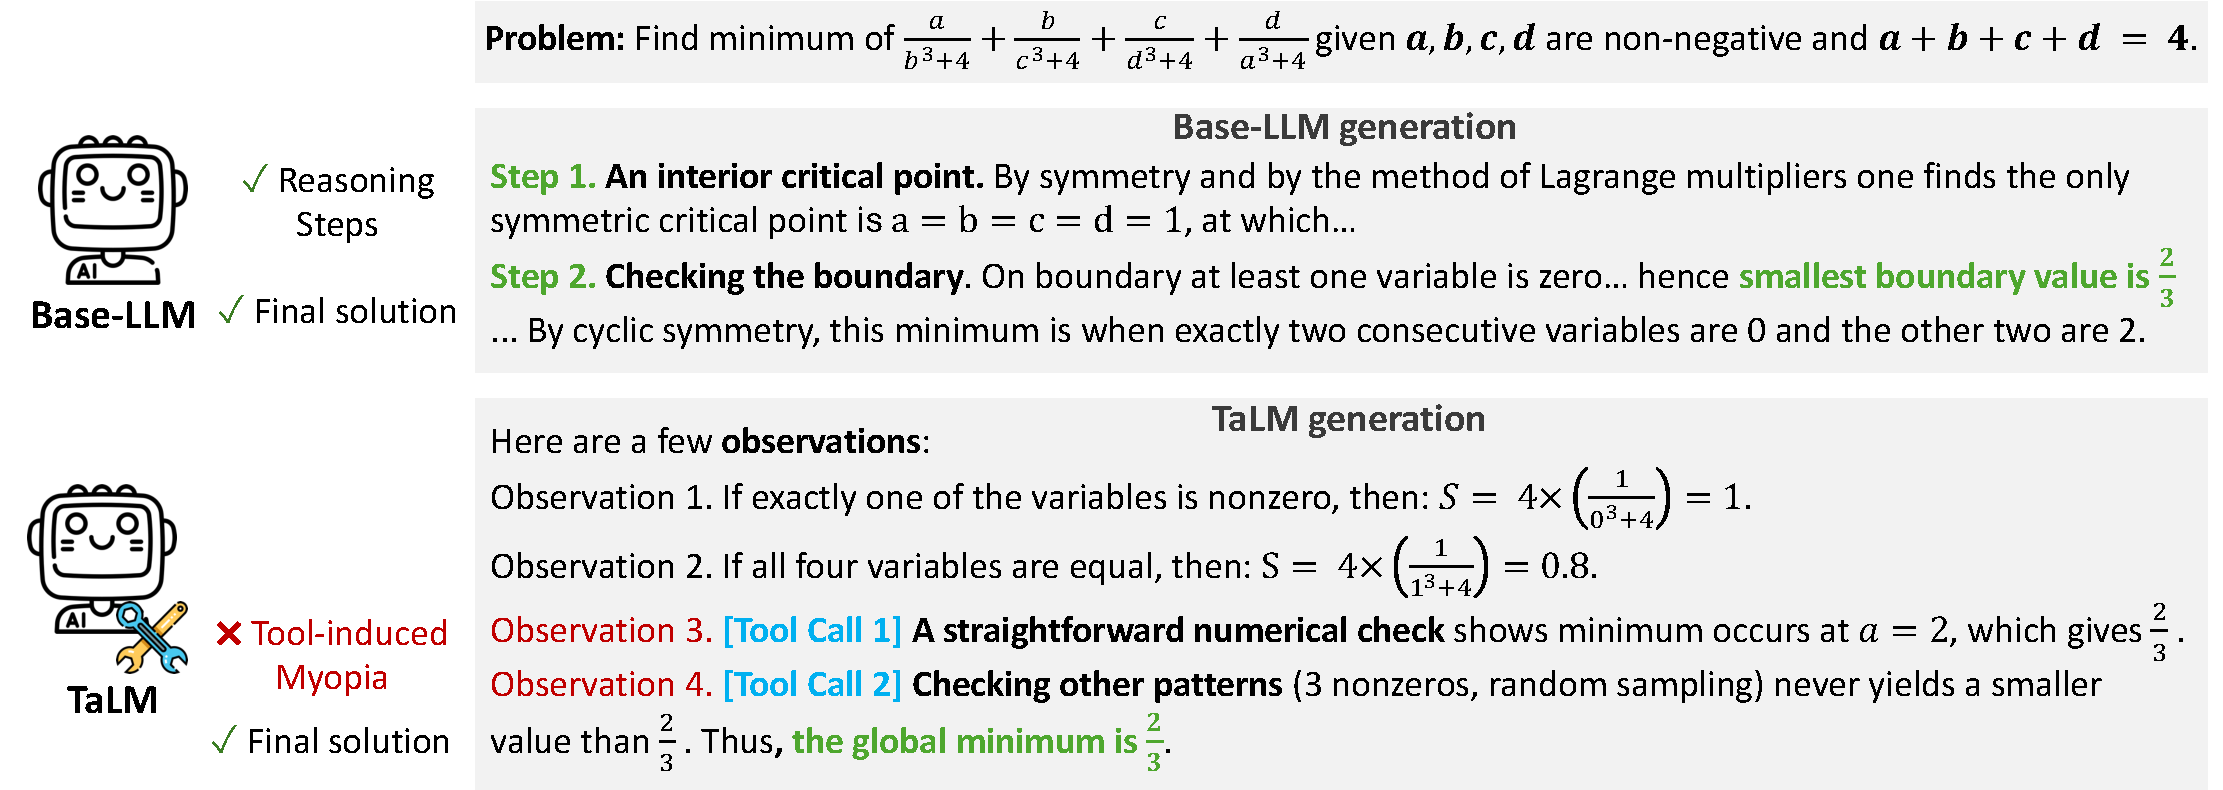
\includegraphics[width=0.98\linewidth]{figures/motivation_new.pdf}
    \caption{Comparison of Base LLM and Tool-augmented LLM (TaLM) reasoning. The Base LLM (top) derives the solution through step-by-step mathematical reasoning, while the TaLM (bottom) relies on \textbf{empirical checks} and multiple tool calls to search for the minimum, a failure mode characteristic of Tool-Induced Myopia (\task). 
    % \pouya{instead of 1,2, 3, 4, say step 1, step 2 ..... also on top of gray boxes maybe say LLM generation and TALM generation} \estevam{can we have this figure on top of the second page, instead of the third? Also, in the figure, should we add ``incomplete'' to the text ``Based on empirical checks'; --> ``Based on incomplete empirical checks''?}
    }
    \label{fig:example}
    \postspace
    \minipostspace
\end{figure*}


% \pouya{"treat computations as substitutes for reasoning" is what our hallucination (TIM) is show. tool overuse and cognitive offloading is not show the substitution . Even based on the two cited papers: overuse = "model’s inability to recognize when
% its internal knowledge is sufficient. This not only
% leads to unnecessary resource consumption but can
% also confuse the model, ultimately degrading performance." and cognitive offloading = "On the one hand, frequent and unnecessary tool calls incur substantial
% computational and temporal overhead, as executing tools - especially at scale - demands significant
% infrastructure and increases operational costs, limiting deployment feasibility. On the other hand,
% extensively rely on external tools may hinder the development and utilization of its own internal
% reasoning capabilities". use similar terms to what they used instead of substitute.)}

% as well as to tool overuse that induces cognitive offloading—a behavior in which the LM over-relies on external tools and treats them as substitutes for reasoning~\citep{qian-etal-2025-smart, wang2025actingreasoningmoreteaching}. 

% Prior studies have primarily divided \textit{tool hallucinations}, where models either select inappropriate tools or misuse them \cite{10.5555/3737916.3741936, xu2025reducingtoolhallucinationreliability}. In contrast, our work investigates post-execution misbehavior, i.e., cases where the correct tool is selected and executed successfully, yet the LM’s reasoning remains flawed. Previous research suggests that conflicts between parametric and non-parametric knowledge can induce hallucinations ~\citep{sun2025redeepdetectinghallucinationretrievalaugmented}, and that factual errors in retrieved information (e.g., legal documents) can propagate to model outputs~\citep{magesh2024hallucinationfreeassessingreliabilityleading}. Other studies show that granting LMs unrestricted access to external tools can encourage tool overuse and lead to cognitive offloading, wherein models defer reasoning to external computations~\citep{qian-etal-2025-smart, wang2025actingreasoningmoreteaching}.

% In this work, we control for all previously studied sources of tool-related failure \---namely, the tool is correctly invoked and executed\--- and introduce \textit{a new family of hallucinations} that emerges under these ideal conditions. \pouya{instead say: In this work, to ensure tools are invoked and executed correctly, we focus exclusively on the Python/Code Interpreter tool---allowing strictly controlled tool-execution settings with correct invocation, error-free runs, intended outputs, and removal of known tool-related confounds---and demonstrate that a new family of hallucinations still arises under these ideal conditions.} 

In this work, we focus exclusively on the Code Interpreter tool for mathematical problem solving to ensure strictly controlled tool use, with correct invocation and error-free execution. Our design avoids confounds introduced by multi-tool settings, such as API failures, interface mismatches, retrieval drift, or external data quality issues~\citep{zhong2025complexfuncbench, faghih2025tool, maekawa2025towards, han2025search}, thereby enabling a controlled investigation. Despite these idealized conditions, we identify a new class of hallucinations, which we term \textbf{T}ool-\textbf{I}nduced \textbf{M}yopia (\task): a failure mode where access to an external tool (e.g., a Code Interpreter) causes the model to narrow its reasoning to what the tool can compute, rather than leveraging its full internal reasoning capabilities. \task{} erodes user trust, as correct final answers can conceal flawed, tool-dependent reasoning.

% In this work, we exclusively focus on the Code Interpreter tool for mathematical problem solving to ensure that tools are both invoked and executed correctly. This setup allows for strictly controlled execution conditions, including correct tool invocation, error-free runs, and intended outputs, 
% % and the removal of known tool-related confounds, 
% while avoiding confounds from multiple tools that would undermine a controlled investigation (e.g., API failures, interface mismatches, retrieval drift, or external data quality issues \citep{zhong2025complexfuncbench, faghih2025tool, maekawa2025towards,han2025search}). We demonstrate that a new family of hallucinations still emerges under these idealized conditions.
% We term this type of hallucination \textbf{T}ool-\textbf{I}nduced \textbf{M}yopia (\task): a failure mode in which access to an external tool (e.g., a Code Interpreter) causes the model to narrow its reasoning to what the tool can compute, rather than utilizing its full internal reasoning capabilities. 

Figure~\ref{fig:example} illustrates this behavior: with Code Interpreter access (TaLM response), the model repeatedly performs \textbf{empirical checks} instead of producing the required reasoning steps generated by the same model without tools (Base-LLM response). Although the tool is correctly invoked and returns valid outputs, the model’s reasoning depth is reduced. Importantly, existing evaluation approaches fail to capture this failure mode. Final-answer accuracy cannot detect it, since both responses are correct, and step-level logical-consistency metrics \citep{lightman2023letsverifystepstep, zheng-etal-2025-processbench, xiareasoneval, liu2025enhancingmathematicalreasoninglarge} also fail because the reasoning remains superficially coherent despite skipping essential logical steps. As a result, exposing \task requires richer, multi-dimensional evaluation of how models reason under tool use.

% \task{} has significant real-world implications. Models achieving correct answers through opaque reasoning appear reliable but are unsafe in practice; they mislead users about actual reasoning capabilities and erode trust in deployed systems.

% This phenomenon has significant real-world implications. Models that reach correct answers through flawed or opaque reasoning may appear reliable during evaluation but remain unsafe in practice and promote a misleading impression of reasoning ability. Such spurious correctness can mislead users, propagate errors, and erode trust. Assessing how a model arrives at an answer is as important as verifying that the answer itself is correct\farima{a shorter version: \task{} has significant real-world implications. Models achieving correct answers through opaque reasoning appear reliable but are unsafe in practice; they mislead users about actual reasoning capabilities and erode trust in deployed systems.
% }. 
% \pouya{in this para or next we should mention the fact that using final score accuracy or metrics that check logical consistency step-wise \textbf{alone} will not be enough to capture this type of hallucination}

% Our hypothesize that even correct tool use biases the model’s reasoning process by anchoring it to partial or low-effort solution paths.

% \estevam{Here, I would add a a few more sentences making it even more explicit why this is important. Something like this: This phenomenon has significant real-world implications. Models that reach correct answers through flawed or opaque reasoning may appear reliable during evaluation but remain unsafe in practice and promote a misleading impression of reasoning ability. Such spurious correctness can mislead users, propagate errors, and erode trust. Assessing how a model arrives at an answer is as important as verifying that the answer itself is correct.}\estevam{feel free to make it shorter, if needed.}

To investigate \task, we introduce \dataset, a dataset comprising 1,679 competition-level mathematical problems collected from multiple sources and curated to elicit, measure, and mitigate \task under Code Interpreter access. We specifically target problems for which code-based computation is helpful but not sufficient for a complete solution
(details in Section~\ref{sec:data_curation}). We then quantify reasoning degradation in TaLMs compared to their Base (non-tool) counterparts using a comprehensive suite of reference-free and reference-based metrics (Section~\ref{sec:evaluation_suite}). Our results show that, even when TaLMs produce correct final answers (up to a 19.3 \textit{percentage point} in final performance gains), they often overrely on tool outputs and produce shallower reasoning traces than non-tool models.
% , they often exhibit shallower reasoning chains than base models as a result of relying on tool outputs. 
This degradation intensifies with tool use: as models invoke tools more frequently, their reasoning becomes less coherent. The associated errors also shift from arithmetic mistakes to global reasoning failures involving logic, assumption, and creativity. Finally, our manual audit finds evidence of \task{} in \textasciitilde{}55\% of high-risk model-generated solutions.
% \pouya{the same as absract add a bit more detail and also try avoiding using 'over-reliance'}

% To mitigate this issue, we develop two complementary strategies. First, we propose a prompting intervention that encourages models to treat tools as reasoning aids, recovering reasoning behavior at inference time without retraining. Second, we develop a preference-optimization framework based on Direct Preference Optimization (DPO;~\citealp{10.5555/3666122.3668460}) 
To mitigate this issue, we propose two complementary strategies: (1) a prompting intervention that encourages models to treat tools as reasoning aids, and (2) a DPO-based \citep{10.5555/3666122.3668460} preference-optimization that aligns TaLMs to integrate the Code Interpreter as an assistant that supports, rather than replaces, mathematical reasoning. 
On the evaluation split of \dataset, the fine-tuned TaLM demonstrates improved reasoning behavior and surpasses both the vanilla TaLM (+0.6\%) and the Base LLM (+3.0\%) in final-answer accuracy.
% 
% a preference optimization training regime based on the Direct Preference Optimization (DPO;~\citealp{10.5555/3666122.3668460}) to encourage the model to treat the code interpreter as an assistant that supports, rather than replaces, its own internal reasoning. On the evaluation split of \dataset, the fine-tuned TaLM demonstrates improved reasoning behavior and surpasses both the untrained TaLM (+0.6\%) and the Base LLM (+3.0\%) in overall performance. 
% 
% To evaluate this hypothesis, we study widely-used popular TaLMs in mathematical problem-solving, a domain where reasoning and computation are tightly coupled. We define and study \textbf{T}ool-\textbf{I}nduced \textbf{M}yopia (\task), as a failure mode in which TaLM's access to a tool (e.g., Python) narrows the model’s reasoning to what the tool can compute. Our contributions are three-fold: \textbf{(i)}: a benchmark of mathematical problems for which code-based computation is helpful, but reasoning matters, \textbf{(ii)} an evaluation suite of reference-free and reference-dependent methods that capture TaLM's reasoning behavior beyond final answer accuracy, and \textbf{(iii)} a training-based strategy to mitigaste \task in TaLMs. Concerely, we introduce \dataset, a benchmark of competition-level mathematical problems, from multiple sources, selected based on three criteria: (1) high difficulty, (2) Scope (English, text-only format), and (3) usefulness—but not sufficiency—of code-based computation (details in Section x). Our evaluation data, \dataset, contains 1082 mathematical problems with step-by-step open-ended solutions. We then quantify reasoning degradation in TaLMs relative to their base (no tool use) counterparts using a comprehensive suite of reference-free and reference-dependent metrics (Section x). 
% 
% Our analysis reveals that, even when the final answers within LM-generated solutions are correct, TaLMs often exhibit weaker reasoning and over-reliance on tool outputs compared to base models. Finally, to mitigate this issue, termed \task, we perform alignment tuning via Direct Preference Optimization (DPO; \citep{10.5555/3666122.3668460}), teaching the model to treat the code interpreter as an assistant rather than a crutch. Using the same evaluation data and suite, we find that the fine-tuned TaLM demonstrates improved reasoning quality and outperforms both its TaLM and base variants.
% 
In summary, our key contributions are:
% \farima{provide some results and insights here too}:
\begin{itemize}
\item \textbf{Tool-Induced Myopia}: We identify \task, a new class of TaLM hallucinations where tool access reduces reasoning depth even under idealized tool-use conditions.
\item \textbf{Benchmark and Evaluation}: We introduce \dataset{}, a competition-level math benchmark with open-ended solutions, along with a multi-dimensional evaluation suite that reveals when and why \task{} emerges and guides safer tool integration.
\item \textbf{Mitigation}: We propose a training-free prompting method and a preference-optimization fine-tuning approach that reduce \task and improve reasoning depth in TaLMs.
\end{itemize}
% \begin{itemize}
% \item \textbf{Tool-induced Myopia}: We uncover a new class of TaLM hallucinations called \task. We demonstrate that, even under ideal tool-use conditions, LLMs exhibit a systematic failure mode in which tool access suppresses internal reasoning and induces tool-driven shortcuts.
% \item \textbf{Evaluation Benchmark:} To surface \task, we introduce \dataset{}, a dataset of competition-level mathematical problems with step-by-step open-ended solutions, where coding can assist in problem solving. We then provide a multi-dimensional evaluation suite that comprehensively measures the reasoning behavior of TaLM compared to its no-tool counterpart. Our evaluation yields actionable insights into when and why \task{} emerges and guides safer tool integration. 
% \item \textbf{Mitigation Strategies:} We propose two complementary mitigation approaches: (i) a training-free prompting method and (ii) a preference-optimization-based fine-tuning regime, both reduce \task and improve reasoning depth in TaLMs.
% \end{itemize}

\section{Tool-induced Myopia}
% We define \textbf{Tool-Induced Myopia (\task{})} as a type of hallucination where access to a tool (e.g., Code Interpreter) narrows the model’s reasoning to what the tool can compute, which may result in a shift from step-by-step reasoning to exploratory, tool-driven search. 
We define \textbf{Tool-Induced Myopia (\task{})} as a type of hallucination that arises in a controlled tool-use setting where the task requires substantial reasoning beyond what the tool alone can provide. In particular, we study competition-style mathematical problem solving with access to a Code Interpreter under two assumptions: (i) tool invocation is correct, and (ii) execution is error-free.
In practice, it substitutes enumeration for proof, skips necessary derivations, mistakes empirical checks for universal guarantees (e.g., brute-force search), and may prematurely stop once code returns a plausible output. 
Note that using code solely for precise computation (e.g., evaluating a determinant or numerically finding a root), while also providing the necessary derivations, is \textbf{not} considered \task{}. 
Figure \ref{fig:example} illustrates \task{}: the Base-LLM solves the problem through step-by-step mathematical reasoning, whereas the TaLM shifts to an exploration-based approach, using empirical observations from internal computation and Code Interpreter to reach the correct answer through numerical search. \task{} degrades reasoning by overrelying on tool outputs in place of the reasoning needed to justify the full solution.
Notably, the TaLM in Figure~\ref{fig:example} still produces the correct final answer via a logically coherent yet incomplete sequence of steps. 
% Hence, evaluations based solely on final-answer accuracy or stepwise logical consistency would miss this hallucination and inflate model performance.
To expose \task{}, we next introduce an evaluation benchmark and a suite of targeted metrics.


\section{Evaluating \task in Language Models}
\subsection{\dataset{}}
\label{sec:data_curation}
We focus on the domain of mathematical problem solving, where reasoning and computation are tightly coupled, and evaluate LLMs under two settings: with and without access to a Python Code Interpreter. We collect English, text-only competition-level math problems from multiple sources, summarized in Table~\ref{tab:data_sources_and_stats}. To mitigate data contamination, we restrict AIME \citep{AIME20242025} to 2024–2025 problems. From Omni-Math \citep{gao2024omnimathuniversalolympiadlevel}, which provides difficulty ratings (1-10 scale), we retain only problems with difficulty $\geq5$, as frontier LLMs have already saturated performance on easier problems \citep{gpt5, claudeopus4andsonnet4}. Finally, we use the full set of problems from OlympiadBench \citep{he-etal-2024-olympiadbench} and OlympicArena \citep{huang2024olympicarena}.
% , llama4models}.
% \pouya{why did we only focus on hard problems?}

To elicit \task{} in TaLMs more effectively, we target problems for which Python code is \textit{helpful but not sufficient}. This setting creates a natural opportunity for tool use, while still \emph{requiring} reasoning over tool outputs to derive a solution. To identify such cases, we adopt an LLM-as-a-judge protocol~\citep{gu2025surveyllmasajudge} to assess each problem along two dimensions: \textbf{(1) Python Usefulness}: whether Python code helps solve the problem; and \textbf{(2) Python Sufficiency}: whether Python code alone, without additional LLM reasoning, is sufficient to fully solve the problem. Appendix~\ref{appendix:data_curation} provides the filtering prompt and a manual validation of the judge.

Table~\ref{tab:data_sources_and_stats} summarizes the resulting statistics by source. Our final dataset comprises 1,679 competition-level problems with step-by-step reference solutions: 1,000 problems (\textasciitilde{}60\%, distributed across sources and problem difficulties) for evaluation, and the rest for TaLM training (10\% development, 90\% DPO fine-tuning; see Section~\ref{sec:talm_tuning}).

% We use 64.4\% of problems (distributed over different sources and difficulties) for evaluation and the remainder for TaLM training (Section~\ref{sec:talm_tuning}). Our final evaluation dataset contains 1,082 (\pouya{shouldn't be 1679}) competition-level problems paired with step-by-step reference solutions.


% \begin{table}[t]
% \centering
% \resizebox{0.49\textwidth}{!}{
% \begin{tabular}{lccc}
% \toprule
% \textbf{Source} & \textbf{Total} & \textbf{Useful \& Not Sufficient} & \textbf{Eval Split (\%)} \\
% \midrule
% AIME$^{*}$ \citep{AIME20242025} & 60 & 13 &  61.5\\
% OlympiadBench \citep{he-etal-2024-olympiadbench} & 674 & 171 &  64.9\\
% OlympicArena \citep{huang2024olympicarena} & 169 & 47 &  53.2\\
% Omni-Math \citep{gao2024omnimathuniversalolympiadlevel} & 2569 & 1448 &  64.8 \\
% \rowcolor{green!10}
% \textbf{\dataset} & - & \textbf{1679} &  \textbf{64.4}\\
% \bottomrule
% \end{tabular}
% }
% \caption{Sources and statistics of competition-level math problems included in the \dataset{} benchmark. $^*$Only AIME 2024–2025 problems included.}
% \label{tab:data_sources_and_stats}
% \postspace
% \end{table}

\begin{table}[t]
\centering
\small
% \resizebox{0.49\textwidth}{!}{
\begin{tabular}{lccc}
\toprule
\textbf{Source} & \textbf{Total} & \textbf{U but not S} & \textbf{Eval (\%)} \\
\midrule
AIME$^{*}$& 60 & 13 &  23.1\\
OlympiadBench& 674 & 171 &  52.0\\
OlympicArena& 169 & 47 &  12.8\\
Omni-Math& 2569 & 1448 &  62.3 \\
\rowcolor{green!10}
\textbf{\dataset} & - & \textbf{1679} &  \textbf{59.5}\\
\bottomrule
\end{tabular}
% }
\caption{Sources and statistics of competition-level math problems included in the \dataset{} benchmark (containing problems where Python is Useful but not Sufficient). $^*$Only AIME 2024–2025 problems are included.}
\label{tab:data_sources_and_stats}
\postspace
\end{table}


% \subsection{Evaluation Suite}
% After curating the dataset, we need reliable methods to capture the \task problem in TaLMs. Previous work mostly rely on outcome based methods which look at the final answer performance. However, recent work shows that we need to evaluate the reasoning behavior of LMs beyond final answer accuracy, and thus, process-based evaluation methods have emerged. In this work, instead of having a single metric to capture the \task issue in LMs, we look at a suite of reference-dependent and reference-free techniques to capture this phenomenon. Concretely, in what comes next, we detail the evaluation methods we used to capture \task. 
% \subsubsection{Process Reward Models}
% \subsubsection{Win Rate}
% \subsubsection{Miss Rate}
% \subsubsection{Final answer performance}

\subsection{Evaluation Suite}
\label{sec:evaluation_suite}
Evaluating LLMs' mathematical reasoning has traditionally relied on outcome-based evaluation, most predominantly final-answer accuracy~\citep{10.1145/3773985, ahn-etal-2024-large}. However, recent studies~\citep{mondorf2024accuracyevaluatingreasoningbehavior, yee2024faithful} have shown that LLMs can reach a correct final answer despite flawed reasoning.
% , likely due to outcome-only supervision during training~\citep{lightman2023letsverifystepstep}. 
This gap has motivated a shift toward process-based evaluation, which assesses LLMs' \textit{reasoning behavior} rather than their task performance.

Process-based approaches span two major families. \textit{Reference-free} methods do not rely on gold reasoning traces and instead assess reasoning behavior via mechanisms such as self-consistency \cite{liu2025enhancingmathematicalreasoninglarge}, or pairwise comparison (e.g., win rate \citep{chen2025learningreasonfactuality, kim_2024_toolllm}). 
% These methods are scalable and useful even when no ground-truth exists. 
In contrast, \textit{reference-dependent} approaches evaluate reasoning against a gold step-by-step solution, enabling fine-grained detection of invalid, missing, or inconsistent steps \citep{yan2025verifybench, chernyshev2025u}.
% \farima{i guess this also needs a citation but i couldn't find any in the context of reasoning}. 
A recent line of work extends this idea via process reward models (PRMs) to score partial solutions step by step, providing a learned measure of reasoning soundness without requiring gold supervision~\citep{lightman2023letsverifystepstep, zheng-etal-2025-processbench, li-etal-2025-fg}. 

As illustrated in Figure~\ref{fig:example}, neither final-answer accuracy nor unidimensional process-based metrics (e.g., PRM scores alone) are sufficient to expose \task in TaLMs: the model may output the correct answer and generate seemingly coherent reasoning steps while still exhibiting degraded reasoning under tool use. This motivates the need for a multi-dimensional evaluation suite that jointly captures: \textbf{(i)} task outcome, \textbf{(ii)} counterfactual impact of tool use, \textbf{(iii)} divergence from ground truth reasoning traces, and \textbf{(iv)} step-level logical consistency. Next, we introduce these four evaluation dimensions and clarify why each one is necessary, yet insufficient on its own, for diagnosing \task.
% Our evaluation suite integrates \textbf{reference-dependent} and \textbf{reference-free}, and PRM techniques to holistically characterize the \task{} phenomenon. Below, we detail the four complementary evaluation dimensions used in this work \pouya{we need a bit of motivation why these four give a good idea about TIM. REMINDER: aslo in each one we should say why they are not enough alone}.

\paragraph{Final-Answer Accuracy:}
\label{sec:final_ans_acc}
We first measure final-answer accuracy as the standard measure of task success.  
Although this metric cannot reveal whether a TaLM solved the problem through mathematical reasoning or tool-driven shortcuts, it confirms that \task failure affects reasoning, not task performance. 
% 
For all subsequent metrics which target reasoning behavior, we evaluate models only on problems with correct final answer to isolate the effect of tool use on how the model reasons, rather than whether it succeeds.

\paragraph{Win Rate:}
\label{sec:win_rate}
To assess whether tool use meaningfully affects reasoning behavior, we compare solutions from a TaLM to those of the corresponding Base (non-tool) LLM. Following prior work showing that LLMs can reliably approximate human preferences~\citep{10.5555/3666122.3668142, chen2025learningreasonfactuality}, we use an LLM judge with a rubric adapted from~\citet{petrov2025proofbluffevaluatingllms} covering four error types: (1) \textit{logic errors} (logical fallacies or unjustified leaps), (2) \textit{assumption errors} (unsupported or incorrect assumptions), (3) \textit{creativity errors} (invalid solution strategies), and (4) \textit{algebra/arithmetic errors} (critical symbolic or numeric mistakes). 
To avoid order bias, we randomize the presentation order of TaLM and Base-LLM solutions~\citep{shi2025judgingjudgessystematicstudy}.
The judge then selects the solution with fewer errors as the winner (prompt in Appendix~\ref{appendix:winrate_prompt}).

% We conduct pairwise comparisons between solutions from TaLMs and their corresponding no-tool LLMs, which we refer to as the base models. 
% Following the success of LLMs to approximate human preference ~\citet{10.5555/3666122.3668142, chen2025learningreasonfactuality}, an LLM judge is prompted to select the solution with higher-quality reasoning based on a set of error categories inspired by~\citep {petrov2025proofbluffevaluatingllms}. Our rubric evaluates multiple error types, including: (1) \textit{logic errors} (logical fallacies or unjustified leaps), (2) \textit{assumption errors} (unsupported or incorrect assumptions), (3) \textit{creativity errors} (invalid solution strategies), and (4) \textit{algebra/arithmetic errors} (critical symbolic or numeric mistakes). The evaluation prompt is provided in Appendix~\ref{appendix:winrate_prompt}.

\textit{Win Rate} measures the proportion of comparisons in which the TaLM solution is preferred (and vice versa). A lower Win Rate indicates tool access \emph{harms} the LLM's reasoning behavior. This comparison-based setup reduces single-judge bias~\citep{liu-etal-2025-verifact, fatahi-bayat-etal-2025-factbench} and captures the counterfactual effect of tool use.

\paragraph{Miss Rate:}
\label{sec:miss_rate}
Inspired by recall-based measures in long-form factuality evaluation \citep{safe, liu-etal-2025-verifact}, we define \textit{Miss Rate} as the proportion of reasoning steps in the ground-truth solution that are absent from the model-generated solution, i.e., $\frac{|\text{missing steps}|}{|\text{gold steps}|}$. A high Miss Rate indicates that the model abandoned a valid derivation, skipped necessary steps, or replaced reasoning with trial-and-error code execution. Unlike final-answer accuracy, Miss Rate detects invalid reasoning paths even when the model reaches the correct solution. However, this metric may over-penalize a solution when the reference solution(s) do not cover all valid reasoning paths (prompt in Appendix~\ref{appendix:missrate_prompt}).

% We compute the \textit{miss rate}, defined as the proportion of steps that contradict or diverge from the ground-truth reference reasoning.  
% A higher miss rate suggests that the model either abandons a valid strategy prematurely or relies heavily on code-based shortcuts to compensate for weak mathematical reasoning.  
% This metric detects process failures even when the final outcome is correct. However, it suffers in cases where there are multiple solutions to a problem and only one a subset of solutions is covered as ground truth. The evaluation prompt is provided in Appendix~\ref{appendix:missrate_prompt}.

\paragraph{PRM Accuracy:}
\label{sec:prm}
Finally, we evaluate step-level reasoning behavior using a Process Reward Model, specifically \textsc{Qwen2.5-Math-7B-PRM800K}~\citep{zheng-etal-2025-processbench}, trained on $\sim$800K annotated mathematical steps. We aggregate step-level scores to obtain an overall correctness score for each solution. However, while PRMs evaluate step correctness, they may fail to detect reasoning shortcuts where code outputs replace derivations, as they lack a holistic view of the solution. In our analysis, we use PRM scores primarily to compare Base-LLM and TaLM solutions, and Appendix~\ref{appendix:prm_stability} shows that this comparative signal remains stable under moderate perturbations. 
% As our analysis uses PRM scores comparatively between Base-LLM and TaLM solutions, we additionally stress-test this comparison under random step removal; Appendix~\ref{appendix:prm_stability} shows that the comparative signal remains stable under moderate perturbations.
% annotated mathematical reasoning steps to identify erroneous ones. An overall correctness score for a solution is obtained by aggregating these step-level scores. While PRMs assess step-level correctness, they may fail to detect reasoning shortcuts where code outputs substitute for derivation, as they do not capture a holistic view of solution completeness.
% While PRMs detect step-level correctness, they cannot detect reasoning shortcuts when the model simply replaces reasoning with code execution results (since they lack a holistic view of the generated solution), hence they cannot reveal \task alone \pouya{maybe you can add: (because they lack a holistic view of the generated solution))}. 
% However, as PRMs are trained to measure step-level correctness and consistency, they cannot fully capture shortcuts that TaLMs make to reach a final answer. 

These four metrics jointly provide minimal yet complete coverage of \task{}: Final-answer accuracy captures outcomes; Win Rate isolates the tool's counterfactual impact on reasoning behavior; Miss Rate quantifies divergence from valid reference reasoning; and a PRM assesses step-level soundness without relying on the ground truth. This set is sufficient because \task{} exhibits a clear and convergent pattern: final-answer accuracy stays the same or improves in TaLMs, while Win Rate declines, Miss Rate increases, and PRM accuracy drops. This suite both distinguishes \task{} from alternative explanations (e.g., general model weakness or genuinely helpful tool use) and is falsifiable: when tools are removed, the pattern recedes, and when tool reliance is increased, it strengthens. Together, these properties can establish both the existence and mechanism of Tool-Induced Myopia.
% Together, these four evaluation dimensions offer a comprehensive analysis of \task{}, exposing hidden degradations in reasoning that are invisible under traditional outcome-only evaluations and enabling a deeper understanding of when and how tool use hinders logical problem solving. \pouya{remove this, but instead as I said at the begining of this subsection add a bit of reasoning why these four, and how they give "comprehensive analysis of TIM"}

% \subsection{Evaluation Suite}
% \label{sec:evaluation_suite}

% Current methodologies to evaluate LM's mathematical reasoning behavior primarily focus on the final result (outcome). However, previous work shows that within the domain of logical reasoning, LMs can regularly use incorrect reasoning to reach the correct final answer due to different factors (e.g., outcome supervision during training). Therefore, process-based evaluation methods emerged that provide fine-grained signals on the correctness of logical steps within the generated solution response. Generally, in order to do so, two different classes of techniques emerged. The first one is reference-free methods that do not rely on gold solution and evaluate an entire solution using techniques such as or self-consistency measurement over multiple sampled logical steps at each time. Also, techniques such as win rate calculation do not evaluate a model in isolation, but choose a better response given 2 opponents. Such methods are very useful when gold solutions are not available or hard to attain, but reference solutions can guide more reliable evaluation techniques. Finally, there are process-based reward models that have been trained to rank generations and provide feedback during training (cite). We also include a recent, popular reward model in our suite to score intermediate logical steps in LM solutions.   

% Our evaluation suite combines \textbf{reference-dependent} and \textbf{reference-free} methods to holistically characterize the \task{} phenomenon. Below, we describe the four complementary evaluation dimensions used in our study.

% \subsubsection{Final Answer Performance (Outcome-based)}
% First, we report the standard metric of final-answer accuracy.  
% While not sufficient for detecting \task{} on its own, this measure provides important context to interpret process-level degradation. Combined with the other three metrics, it allows us to determine whether correct answers were achieved by robust reasoning or shallow trial-and-error computation.

% \subsubsection{Win Rate}
% We compare pairs of solutions: one from the TaLM and one from the base LM (no tool access).  
% Following a pairwise evaluation framework~\citep{zheng2023judging}, we prompt an LM judge (GPT-5-Thinking) to determine which solution exhibits better reasoning quality. The \textit{win rate} is defined as the percentage of pairwise comparisons in which a model's solution is preferred over its counterpart.  
% This metric directly reveals whether tool access improves or hurts reasoning relative to a baseline with no tool use. Add explanations into how win_rate calculated. (based on these reasoning categories (maybe just say prompt in appendix which is adopted from proof or bluff paper, explain why and cite:
% 1. Logic Errors: Errors due to logical fallacies (e.g. circular reasoning) or unjustified leaps disrupting the reasoning.

% 2. Assumption Error: Errors coming from the introduction of unproven or incorrect assumptions that undermined subsequent steps.

% 3. Creativity Error: Errors resulting from fundamentally incorrect solution strategies due to the inability to identify the correct approach.

% 2. Algebra/Arithmetic Error: Errors arising from critical algebraic or arithmetic miscalculations.)

% \subsubsection{Miss Rate)}
% We also quantify the percentage of reasoning steps that contradict or are inconsistent with the ground-truth reference solution, which we refer to as the \textit{miss rate}.  
% A higher miss rate indicates that the LM either deviates early from a valid reasoning path or unnecessarily relies on code execution to compensate for missing analytical steps.  
% This metric captures divergence in the reasoning process even when the final answer happens to be correct.

% \subsubsection{Process Reward Models}
% To assess the quality of intermediate reasoning, we employ a Process Reward Model (PRM), which scores each reasoning step on its mathematical validity and logical contribution, without access to the ground-truth solution.  
% Higher PRM scores indicate stronger reasoning coherence, whereas lower scores often correlate with tool overuse and shallow reasoning behaviors. We report both \textit{average PRM score} per step and cumulative score per solution.

% \vspace{4pt}
% Together, these four evaluation dimensions enable us to rigorously identify and quantify \task{}, revealing reasoning failures that would remain hidden under traditional outcome-only evaluation protocols.


\section{Experimental Setup}
\label{sec:experimental_setup}
\textbf{Large Language Models:} We evaluate frontier proprietary language models equipped with in-house Code Interpreters. These models can autonomously decide when to invoke tools, allowing us to study tool-augmented reasoning without modifying or intervening in their internal execution pipeline.
% 
We benchmark seven models across three families:
(1) OpenAI GPT-4.1-mini and GPT-4.1 (non-thinking LLMs; \citealp{gpt4.1}), and o4-mini~\citep{o4-mini-model} and GPT-5~\citep{gpt5} (thinking LLMs), (2) Gemini-2.0-Flash (non-thinking; \citealp{gemini-2-model}) and Gemini-2.5-Flash (thinking; \citealp{gemini2.5-flash}), (3) Claude-Opus-4 (thinking; \citealp{claudeopus4andsonnet4}).
% 
% For each family, we evaluate both the base and tool-augmented (Code Interpreter) variants.

\noindent
\textbf{Evaluation Benchmark}: We use the evaluation split of \dataset as our benchmark dataset and apply our four-dimensional evaluation suite to measure reasoning and tool-use behavior. 
% The suite comprises: (1) Final-answer Accuracy, (2) Win Rate (pairwise reasoning comparison), (3) Miss Rate (proportion of missing steps from ground truth), (4) PRM Accuracy (reasoning correctness based on stepwise judgment). 
% We adopt an LLM-as-a-judge protocol with GPT-5 as the judge.
We use GPT-5 as the judge for all LLM-as-a-judge evaluations.
% This enables a comprehensive comparison between TaLMs and their Base counterparts.
% \pouya{we need to cite some previous previous works here to show the trustworthiness of llm as a judge for each metric}

% \begin{table*}[t]
% \centering
% \small
% \renewcommand{\arraystretch}{1.15}
% \begin{tabular}{l l c c c c}
% \toprule
% \textbf{Model} & \textbf{Variant} & \textbf{Final Acc. ($\uparrow$)} & \textbf{Miss Rate ($\downarrow$)} & \textbf{Win Rate ($\uparrow$)} & \textbf{PRM Acc. ($\uparrow$)} \\
% \midrule
% \multirow{2}{*}{GPT-4.1-mini} 
%  & Base & 29.57 & 45.39 & 57.92 & \colorbox{green!10}{92.50} \\
%  & TaLM & 28.47 & 49.34 & 42.08 & 89.61 \\
% \midrule
% \multirow{2}{*}{GPT-4.1} 
%  & Base & 24.12 & 48.10 & 55.17 & 89.27 \\
%  & TaLM & 26.16 & 49.45 & 44.83 & 86.22 \\
% \midrule
% \multirow{2}{*}{o4-mini} 
%  & Base & 44.82 & 45.16 & 48.78 & 84.01 \\
%  & TaLM & 64.33 & 48.02 & 51.22 & 73.81 \\
% \midrule
% \multirow{2}{*}{GPT-5-Thinking} 
%  & Base & 67.10 & \colorbox{green!10}{37.78} & 56.15 & 56.47 \\
%  & TaLM & \colorbox{green!10}{72.18} & 43.69 & 43.85 & 48.79 \\
% \midrule
% \multirow{2}{*}{Gemini-2.0-Flash} 
%  & Base & 24.40 & 53.70 & 52.02 & 64.77 \\
%  & TaLM & 24.77 & 55.93 & 47.98 & 67.54 \\
% \midrule
% \multirow{2}{*}{Gemini-2.5-Flash} 
%  & Base & 45.47 & 39.72 & 53.75 & 80.89 \\
%  & TaLM & 45.66 & 40.85 & 46.25 & 78.54 \\
% \midrule
% \multirow{2}{*}{Claude-Opus-4} 
%  & Base & 27.73 & 50.86 & 41.70 & 78.33 \\
%  & TaLM & 40.39 & 53.19 & \colorbox{green!10}{58.30} & 57.89 \\
%  \midrule
% % \multirow{2}{*}{\textbf{Average}} & Base & 39.25 & \textbf{0.45} & \textbf{52.60} & \textbf{77.99} \\
% %                  & TaLM & \textbf{43.60} & 0.48 & 47.40 & 74.09 \\
% \multirow{2}{*}{\textbf{Average}} & Base & 37.32 & \textbf{45.82} & \textbf{52.50} & \textbf{78.89} \\
%                                  & TaLM & \textbf{43.71} & 48.36 & 47.50 & 71.77 \\
% \bottomrule
% \end{tabular}
% \caption{Performance of base LLMs and TaLMs across four reasoning metrics. The best score in each column is highlighted in \colorbox{green!10}{green}. The average row shows a consistent pattern: TaLMs achieve higher Final Answer Accuracy (Final Acc.), but base LLMs exhibit better reasoning behavior—lower Miss Rate, higher Win Rate, and higher PRM Accuracy, reflecting the presence of \task{}.
% % \farima{can show miss rate in \% as well to be consistent with other metrics.} \pouya{+1}
% }
% \label{tab:main_results}
% \postspace
% \end{table*}

\begin{table*}[t]
\centering
\small
\renewcommand{\arraystretch}{0.9}
\begin{tabular}{l l c c c c}
\toprule
\textbf{Model} & \textbf{Variant} & \textbf{Final Acc. ($\uparrow$)} & \textbf{Miss Rate ($\downarrow$)} & \textbf{Win Rate ($\uparrow$)} & \textbf{PRM Acc. ($\uparrow$)} \\
\midrule
\multirow{2}{*}{GPT-4.1-mini} 
 & Base & 30.0 & 45.7 & \colorbox{green!10}{58.6} & \colorbox{green!10}{93.0} \\
 & TaLM & 28.7 & 49.9 & 41.4 & 88.9 \\
\midrule
\multirow{2}{*}{GPT-4.1} 
 & Base & 24.6 & 48.1 & 54.4 & 88.6 \\
 & TaLM & 27.0 & 49.9 & 45.6 & 85.9 \\
\midrule
\multirow{2}{*}{o4-mini} 
 & Base & 45.1 & 45.5 & 49.0 & 73.6 \\
 & TaLM & 64.4 & 47.6 & 50.9 & 67.9 \\
\midrule
\multirow{2}{*}{GPT-5-Thinking} 
 & Base & 67.5 & \colorbox{green!10}{38.8} & 56.0 & 57.5 \\
 & TaLM & \colorbox{green!10}{71.9} & 43.8 & 44.0 & 50.2 \\
\midrule
\multirow{2}{*}{Gemini-2.0-Flash} 
 & Base & 24.3 & 54.2 & 52.7 & 65.0 \\
 & TaLM & 25.1 & 56.6 & 47.3 & 68.5 \\
\midrule
\multirow{2}{*}{Gemini-2.5-Flash} 
 & Base & 45.4 & 40.2 & 54.6 & 81.5 \\
 & TaLM & 45.7 & 40.9 & 45.4 & 78.8 \\
\midrule
\multirow{2}{*}{Claude-Opus-4} 
 & Base & 28.0 & 50.9 & 41.3 & 77.9 \\
 & TaLM & 40.5 & 52.8 & \colorbox{green!10}{58.6} & 57.8 \\
 \midrule
% \multirow{2}{*}{\textbf{Average}} & Base & 39.25 & \textbf{0.45} & \textbf{52.60} & \textbf{77.99} \\
%                  & TaLM & \textbf{43.60} & 0.48 & 47.40 & 74.09 \\
\multirow{2}{*}{\textbf{Average}} & Base & 37.8 & \textbf{46.2} & \textbf{52.4} & \textbf{76.7} \\
                                 & TaLM & \textbf{43.3} & 48.8 & 47.6 & 71.1 \\
\bottomrule
\end{tabular}
% \vspace{-1mm}
\caption{Performance of Base-LLMs and TaLMs across four evaluation metrics. Best score in each column is highlighted in \colorbox{green!10}{green}. On average, TaLMs achieve higher Final-answer Accuracy (Final Acc.), yet Base-LLMs exhibit greater reasoning depth, confirming the presence of \task{}.
% \farima{can show miss rate in \% as well to be consistent with other metrics.} \pouya{+1}
}
\vspace{2mm}
\label{tab:main_results}
\postspace
\end{table*}

\section{Results and Analyses}
% \pouya{in discussion part of this section we should point out to the fact that the reason we only see moderate better perf in base vs tool, are possibly because of several reasons like the fact that not all samples prone (despite out filtering approach) to this type of error, evaluation metric alone are not perfect to capture them, even looking at the current leader board having tool only moderate improve the performance which impact out moderate result too, also if we do breakdown based on different category we will se mor gap.}
% In this section, we first evaluate Base-LLMs and their tool-augmented counterparts (TaLMs) using our four-dimensional evaluation suite in Section~\ref{sec:benchmarking_results}. Section~\ref{sec:tool_call_and_tim} further examines how the severity of \task{} in the LLM-generated solution changes as the number of tool calls increases. We also investigate whether the complexity of TaLM-generated code correlates with the degree of reasoning hallucination in their solutions in Section~\ref{sec:code_complexity}.
% Next, we apply the error taxonomy introduced in Section~\ref{sec:win_rate} to analyze the prevalent error types that occur when LLMs have access to a Code Interpreter compared to Base-LLMs (Section~\ref{sec:error_type_analysis}). 
% Since \dataset encourages but does not guarantee tool use, in Section~\ref{sec:tool_invocation_rate} we analyze the frequency of tool invocation for TaLMs.
% Finally, Section~\ref{sec:quality_analysis} presents a qualitative analysis validating that the high-risk solutions flagged by our evaluation suite indeed exhibit \task{} behaviors.

In this section, we first evaluate Base-LLMs and their tool-augmented counterparts (TaLMs) using our four-dimensional evaluation suite (Section~\ref{sec:benchmarking_results}). We then examine how the severity of \task{} varies with the number of tool calls (Section~\ref{sec:tool_call_and_tim}) and analyze whether the complexity of TaLM-generated code correlates with reasoning hallucinations (Appendix ~\ref{appendix:code_complexity}).
Next, we apply the error taxonomy from Section~\ref{sec:evaluation_suite} to characterize error types introduced by tool access (Section~\ref{sec:error_type_analysis}), and analyze tool invocation frequency given that \dataset{} encourages, but does not guarantee, tool use (Section~\ref{sec:tool_invocation_rate}).
Finally, Section~\ref{sec:quality_analysis} presents a qualitative analysis confirming that solutions flagged as high risk by our metrics indeed exhibit \task{} behavior.


\subsection{Base-LLMs Show Stronger Reasoning Despite Lower Accuracy}
\label{sec:benchmarking_results}
Our benchmarking results on the evaluation set of \dataset are presented in Table~\ref{tab:main_results}. We report Final-answer Accuracy, Miss Rate, Win Rate, and PRM Accuracy across the Base and TaLM variants of seven LLMs. The results reveal a consistent pattern characteristic of \task{}: although \textbf{TaLMs achieve higher Final-answer Accuracy, Base-LLMs exhibit stronger mathematical reasoning}, reflected in lower Miss Rates, higher Win Rates, and higher PRM Accuracy on average. Prior work has shown that LLMs can produce the correct final answer despite flawed or incomplete reasoning \citep{mondorf2024accuracyevaluatingreasoningbehavior}. Our findings demonstrate that access to external tools often amplifies this discrepancy. 
% lightman2023letsverifystepstep

Interestingly, the highest PRM scores are achieved by non-thinking GPT-4.1 models compared to their stronger ``thinking'' variants. This is inline with recent findings that step-level reward models struggle to reliably assess long and complex reasoning chains, often conflating fluency with correctness, becoming miscalibrated on stronger models, and generalizing poorly to the longer, self-correcting traces produced by advanced reasoning models~\citep{BambaRewardUA, lee2025rethinkingrewardmodelsmultidomain}.

Finally, we posit that the reasoning gap between Base-LLM and TaLM appears moderate in aggregate because \task{} is partially masked by three factors: (1) our filtering for \task-prone problems, while targeted, is not perfect; (2) existing metrics have limited sensitivity to \task{} hallucinations; and (3) tool use yields only modest accuracy gains for most LLMs. For subsequent analyses, we focus only on solutions with correct final answers.
% We next show that this reasoning gap widens as the number of tool invocations increases.
% However, a breakdown by tool call frequency (Section~X\estevam{remeber to update the reference to the righ section}) reveals that the reasoning gap widens substantially when TaLMs invoke tools more frequently \pouya{(which correlates with increased possibility of TIM)}, providing clearer evidence of the underlying difference \pouya{instead of the underlying difference shouldn't we say TIM}.

\begin{figure*}
    \centering
    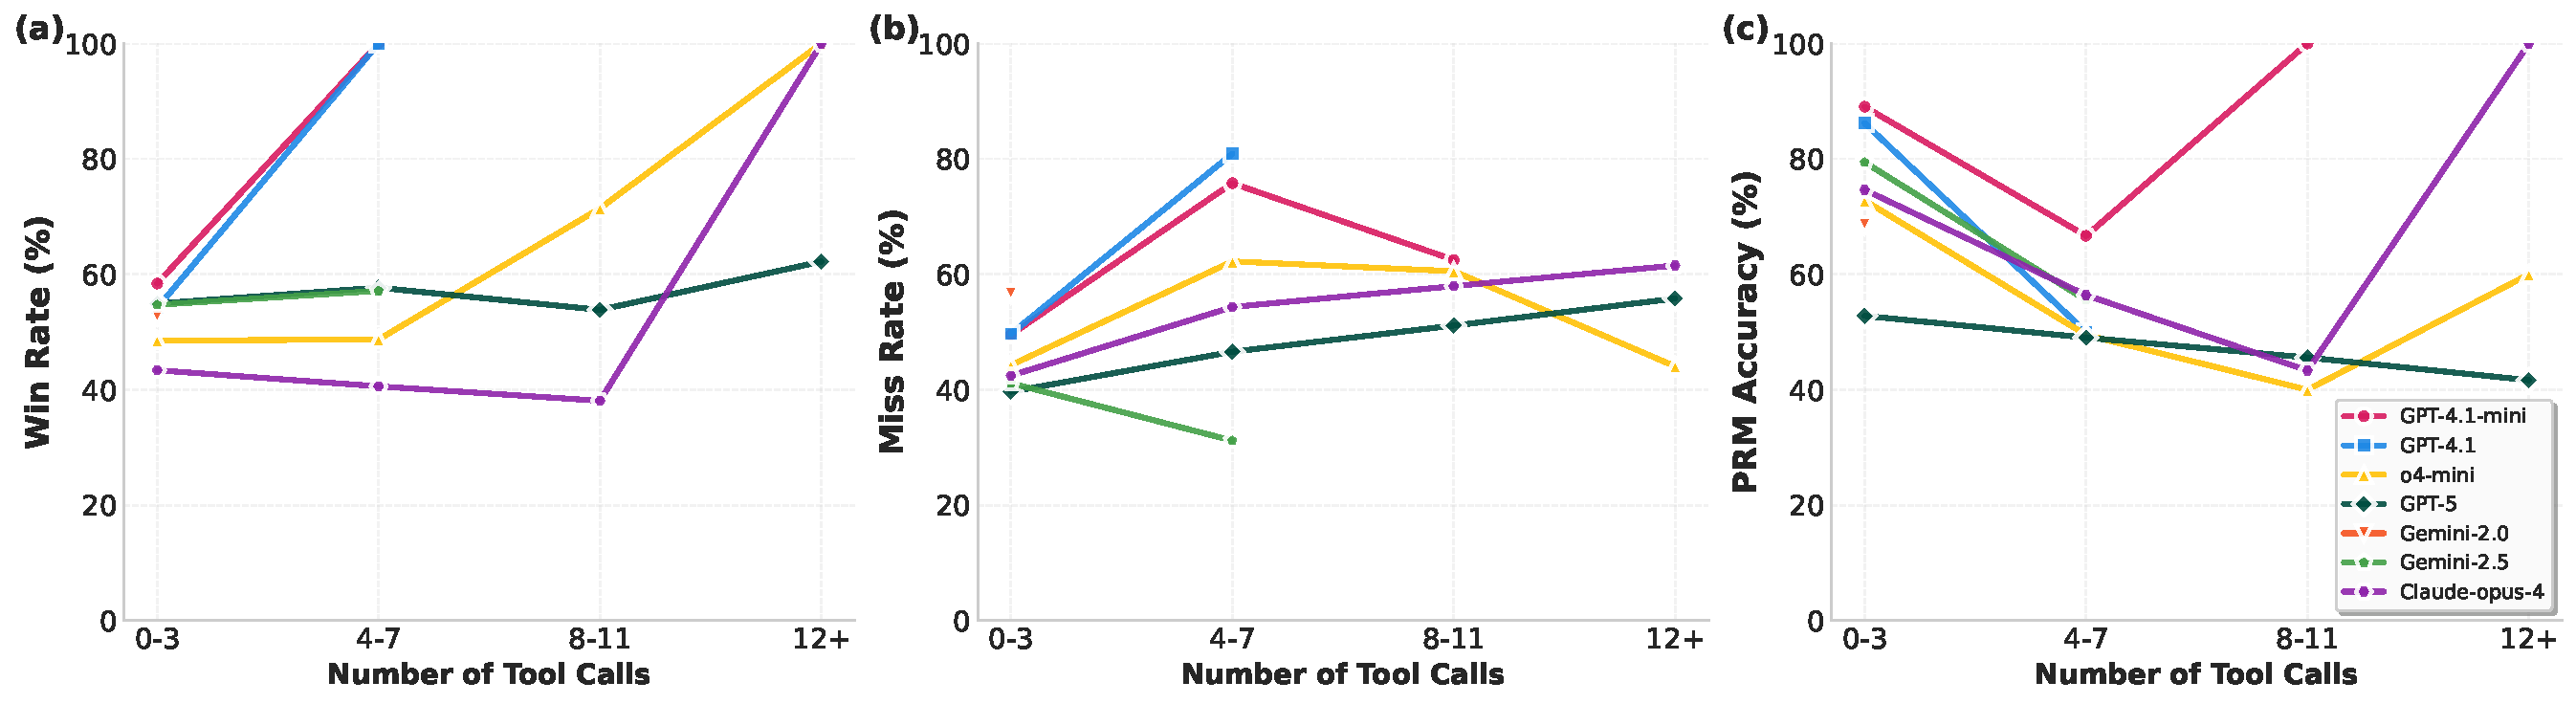
\includegraphics[width=0.98\linewidth]{figures/metrics_combined_new.pdf}
    % \vspace{-1mm}
    \caption{Impact of tool-call frequency on TaLM reasoning. Across tool-call bins (0–3 to 12+), higher tool-call frequency is associated with (a) increased Base-over-TaLM Win Rate, (b) higher Miss Rate, and (c) lower PRM Accuracy, indicating a widening reasoning gap as reliance on tools grows.
    % Across tool-call bins {0–3, 4–7, 8–11, 12+}, increased tool use widens the Base–TaLM gap, with lower Win Rate, higher Miss Rate, and reduced PRM Accuracy for \textsc{TaLM}.
    % Metrics are computed over bins defined by the number of tool calls in model solution: \{0--3, 4--7, 8--11, 12+\}. 
    % \textbf{(a) Win Rate} (higher is better) shows that the Base model more frequently outperforms \textsc{TaLM} as tool usage increases, indicating a widening gap at higher call counts. 
    % \textbf{(b) Miss Rate} (higher is worse) generally rises with additional tool calls, indicating more missing steps in tool-dependent trajectories. 
    % \textbf{(c) PRM Accuracy} (higher is better) typically declines as the number of calls grows.
    % , consistent with increased local inconsistencies over longer chains.
    % Deviations in the 12+ bin are influenced by limited sample sizes.
    }
    % \vspace{-1mm}
    \label{fig:metrics_categorized}
    \postspace
\end{figure*}


\subsection{Base-TaLM Reasoning Gap Widens with Number of Tool Calls}
\label{sec:tool_call_and_tim}

We examine how reasoning behavior varies with tool-call frequency, a key factor underlying \task: as tool reliance grows, models increasingly substitute computation for reasoning. We test whether higher number of calls amplify the Base–TaLM gap when final answers are correct. We group problems into bins based on the number of tool calls in their TaLM-generated solutions: \{0--3, 4--7, 8--11, 12+\}. Figure~\ref{fig:metrics_categorized} shows three consistent trends across most models.
First, the Base model’s \emph{Win Rate} against the TaLM increases with tool-call frequency, indicating degraded reasoning under heavier tool reliance. Second, the \emph{Miss Rate} generally rises with increased tool calls, reflecting greater divergence from reference reasoning. Third, \emph{PRM Accuracy} typically declines as tool calls increase, suggesting that longer, tool-heavy trajectories accumulate step-level errors. Occasional reversals in the 12+ bin are due to limited sample sizes. 
We further verify that this effect is not explained by the syntactic or structural complexity of generated code; detailed analysis shows no correlation between code complexity and \task{} severity (Appendix~\ref{appendix:code_complexity}).

% First, the \emph{Win Rate} of the Base model against \textsc{TaLM} increases with tool call frequency, indicating that reasoning weakens as solutions rely more heavily on tools. 
% Second, the \emph{Miss Rate} 
% % —our measure of reasoning divergence from reference solutions—
% generally increases with more tool usage, reflecting larger deviations from mathematically grounded reasoning. 
% Third, \emph{PRM Accuracy} typically decreases as tool calls grow, suggesting that longer, tool-heavy trajectories accumulate more step-level errors. 
% Occasional reversals in the 12+ bin are due to the limited number of samples in that category.

% We examine how reasoning quality varies with tool-call frequency, a key stressor for \task: as reliance on tools grows, models are more likely to replace deduction with enumeration. Accordingly, we test whether higher call counts yield larger Base–TaLM divergence and degraded metrics (e.g. higher Miss Rates and lower PRM Accuracy) even when final answers are correct.
% In order to do that, we group problems into bins of \{0--3, 4--7, 8--11, 12+\} calls based on the number of calls in their LLM-generated solution. As shown in Figure~\ref{fig:metrics_categorized}, three consistent patterns emerge across most models. 
% First, the \emph{Win Rate} of the Base model against \textsc{TaLM} tends to increase with the number of tool calls, indicating that the performance gap widens as solutions rely more heavily on tools. 
% Second, the \emph{Miss Rate}---our measure of reasoning divergence from gold solutions---generally increases with more tool usage, reflecting more diverged solutions. 
% Third, \emph{PRM Accuracy} typically decreases as the number of tool calls grows, suggesting that longer, tool-heavy trajectories are less likely to remain locally correct at each step. 
% Occasional reversals in the highest bin (12+) are best interpreted with caution due to the small sample size in that category.

\subsection{Tool Use Induces Global Reasoning Errors}
\label{sec:error_type_analysis}
% \pouya{You should have 1-2 sentnces at the begining of each ablation section, motivating why we are doing this experiment and what we want to show. Basically in these 2-3 sentences you should mention why this is correlated with showing TIM happening.}
In this section, we analyze how reasoning error types shift under tool use by comparing TaLM solutions with those of Base-LLMs. 
% Our goal is to probe the core mechanism of \task{}: how reasoning failures changes when a model shifts from mathematical derivation to computation-heavy solutions.
Using the error taxonomy adapted from \citet{petrov2025proofbluffevaluatingllms}, we prompt our LLM judge (GPT-5) to rate each error type on a 1--5 scale, or output \texttt{None} if no error is detected (prompt in Appendix~\ref{appendix:prevalent_error_annotation}). 
% As before, we restrict analysis to cases where \textbf{both} the Base-LLM and the TaLM produce the correct final answer.

Across models, tool use induces a consistent shift in error patterns (Figure~\ref{fig:error_rates_delta}). Logic, assumption, and creativity errors increase in nearly all cases, indicating more unjustified inferences and reasoning shortcuts under tool reliance. In contrast, algebraic and arithmetic errors decrease as computation is delegated to the Code Interpreter, while the rate of error-free solutions also drops. These results show that \task{} is not merely about missing steps, but reflects a fundamental change in how models reason under tool use.

% Across models, we observe a consistent shift in error patterns with tool use (Figure~\ref{fig:error_rates_delta}): logic, assumption, and creativity errors in almost all cases increase, indicating that TaLMs make more unjustified inferences and reasoning leaps when relying on tool outputs. In contrast, algebraic and arithmetic errors decrease, since computation is delegated to Code Interpreter, while the proportion of ``no error'' cases drops, showing that tool access introduces new reasoning flaws even when final answers remain correct. Therefore, \task{} does not simply result in missing steps; rather, it fundamentally reshapes the model's \emph{reasoning behavior}. 
% by increasing logically invalid or unjustified steps even when correctness is preserved.

% Across models, we observe a consistent shift in error patterns after tool use (Figure \ref{fig:error_rates_delta}): logic, assumption, and creativity errors all increase, indicating that TaLMs make more unjustified inferences and leaps in reasoning when relying on tool outputs. In contrast, algebraic and arithmetic errors (Algebra) decrease—since computation is delegated to Python—and the proportion of ``no error'' cases drops, showing that tool access introduces new reasoning flaws even when the final answer remains correct. These results reinforce that \task{} does not simply result in missing steps
% % produce wrong answers \estevam{do we show that TIM produces wrong answers?}
% ; it reshapes the model’s \emph{internal reasoning process}, increasing logically invalid or unjustified reasoning even when the final answer is preserved.

\begin{figure}
    \centering
    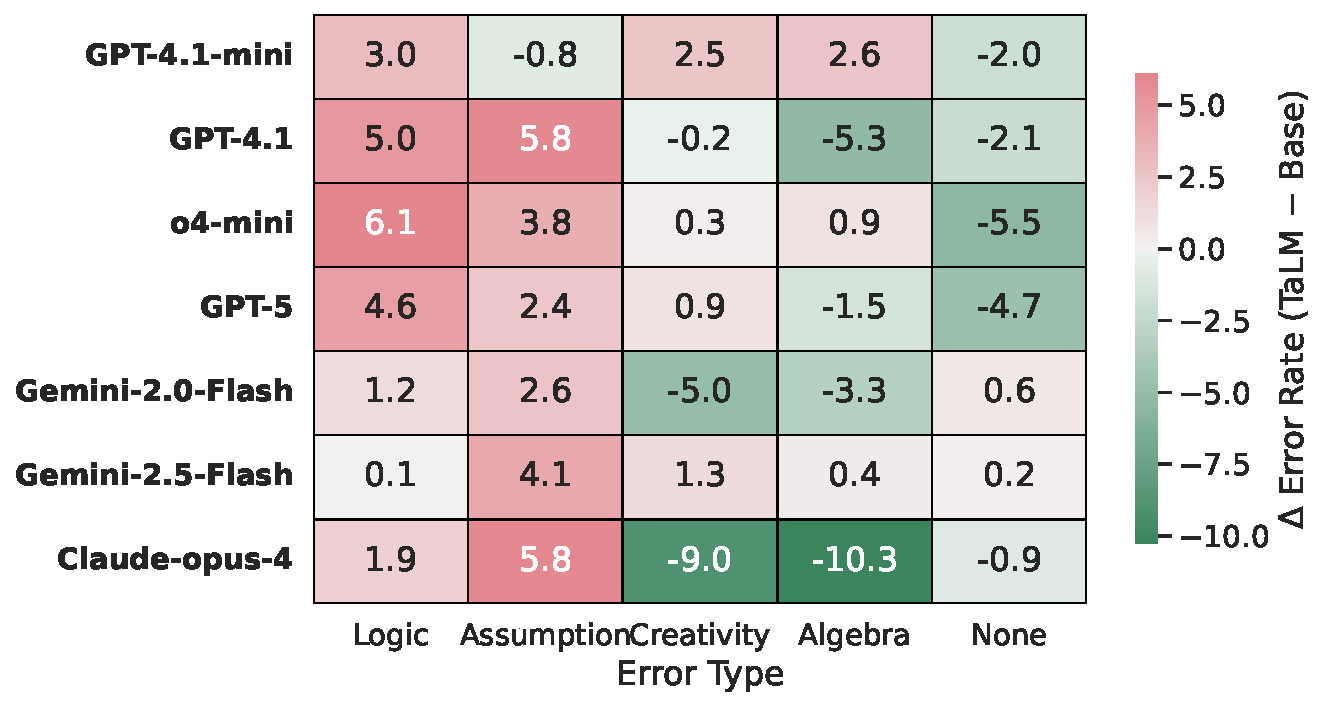
\includegraphics[width=0.98\linewidth]{figures/error_rates_delta_new.pdf}
    % \vspace{-4mm}
    \caption{Change in reasoning error rates after tool use (\(\Delta = \text{TaLM} - \text{Base}\)). Positive values indicate higher error frequency with Code Interpreter access.}
    \label{fig:error_rates_delta}
    % \vspace{-3mm}
    \postspace
\end{figure}


\subsection{Thinking Models Use Code More Often} 
\label{sec:tool_invocation_rate}

Having shown that more tool calls intensify \task{}, we now quantify how often each model invokes the Code Interpreter tool on math problems, providing a ``dose'' measure of \task{} risk. We investigate tool use rates across TaLMs on \dataset, which was curated to encourage code use. Figure~\ref{fig:tool_use_rate} shows the percentage of problems on which each TaLM invoked the Code Interpreter tool. Thinking models exhibit substantially higher tool usage than non-thinking models: Claude-opus-4 achieves the highest rate at 99.8\%, followed by GPT-5 at 73.7\%, while non-thinking models show more modest usage.
% : GPT-4.1-mini (16.4\%), GPT-4.1 (25.9\%), and Gemini-2.0-flash (14.3\%). 
\textbf{On average, thinking models invoke code on 49.7\% more problems.} Given the established relationship between tool-call frequency and \task{} severity (Section~\ref{sec:tool_call_and_tim}), this heavier reliance suggests that thinking models face higher \task{} risk.

\begin{figure}
    \centering
    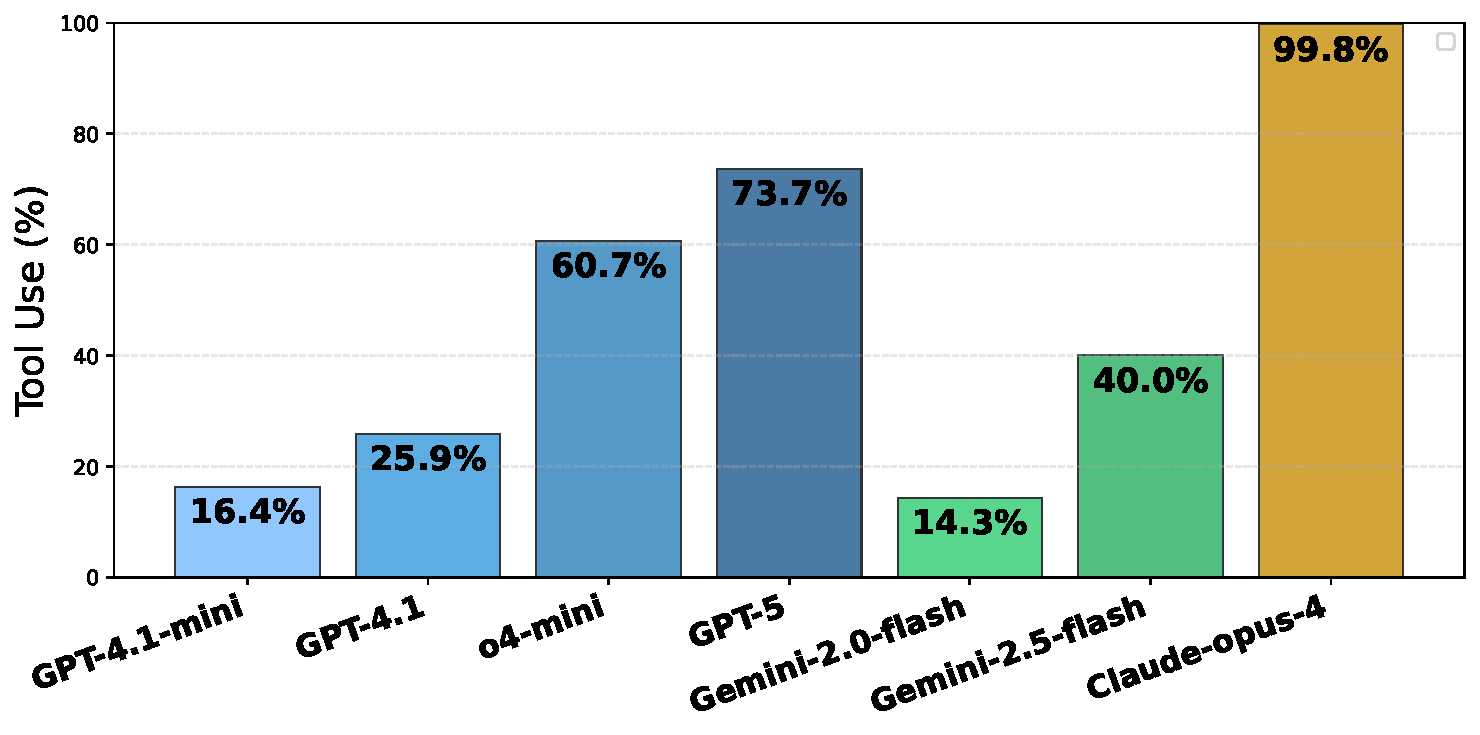
\includegraphics[width=0.98\linewidth]{figures/tool_use_rate_new.pdf}
    \caption{Tool use rate across TaLMs. Thinking TaLMs (GPT-5, o4-mini, Gemini-2.5-Flash) invoke code on \textasciitilde50\% more problems than non-thinking models.
    % use the tool on an average of \textasciitilde{}50\% more problems than non-thinking models.
    }
    \vspace{-3mm}
    \label{fig:tool_use_rate}
\end{figure}

% \pouya{Having shown in the previous section that more Python calls intensify TIM, widening Base–TaLM divergence and degrading metrics, we now quantify how often each model invokes Python on math problems, providing a ``dose'' measure that clarifies TIM risk across models.}
% We investigate how frequently different TaLMs invoke the Python interpreter when solving mathematical problems. During benchmark curation, we filtered for problems where Python would be useful, aiming to encourage tool use. Figure~\ref{fig:tool_use_rate} shows the percentage of problems on which each TaLM invoked the Python interpreter. Thinking models exhibit substantially higher tool use rates compared to their non-thinking counterparts, with GPT-5 achieving the highest rate at 74.1\%, followed by o4-mini at 61.1\%. In contrast, non-thinking models show more modest usage: GPT-4.1-mini (16.6\%), GPT-4.1 (25.1\%), and Gemini-2.0-flash (13.4\%). This demonstrates the heavy reliance of thinking models on tool calls, which in turn can increase the likelihood of \task{} hallucination in their responses.


\subsection{\task{} in Over Half of High-Risk Solutions}
\label{sec:quality_analysis}
We conduct a targeted manual evaluation to validate \task{} qualitatively and identify recurring linguistic cues that precede it. We focus on high-risk TaLM solutions that satisfy three criteria: (1) a correct final answer, (2) Base-LLM solution is preferred over the TaLM solution in Win Rate judgment, and (3) PRM flags errors in the TaLM’s reasoning trace. From this filtered set, we select the top 10 samples per model ranked by Miss Rate to assess \task{} presence and characteristic precursor phrases.

% We focus on high-risk TaLM-generated solutions where: (1) the final answer is correct, (2) the Base-LLM response is preferred over TaLM in Win Rate judgment, and (3) the PRM flags errors in TaLM's reasoning traces. From this filtered set, we select the top-10 samples per model ranked by Miss Rate and examine them to determine whether \task{} is present and identify characteristic precursor phrases.

Across models, \textbf{\task{} appears in 54.3\% of high-risk cases}, demonstrating strong alignment between our automated metrics. Incidence is higher for models with greater tool use (Figure~\ref{fig:tool_use_rate}), such as Claude-Opus-4 and o4-mini, and lower for Gemini models. Less capable models often display explicit precursor cues (e.g., ``one numerically finds,'' ``systematic checks show,'' or ``let's verify programmatically.''), whereas stronger models like GPT-5 silently substitute code outputs for derivations (more details and a list of precursor phrases in Appendix~\ref{appendix:common-precursor-phrases}). These cues are indicative rather than definitive and should be interpreted alongside quantitative metrics.

% Our inspection reveals that \textbf{\task{} appears in 54.3\%
% % \farima{shouldn't we go with the exact number?} 
% of high-risk cases across models}, demonstrating the correlation between \task{} incidence and our automated metrics. \task{} prevalence varies across models: those where tool use has a greater impact on reasoning quality (Table~\ref{tab:main_results}), such as Claude-Opus-4 and o4-mini, exhibit more frequent \task{}, while Gemini models, for which tool use has minimal impact, show lower rates. Notably, less capable models often display explicit linguistic cues immediately before \task{} instances, such as ``one numerically finds,'' ``systematic checks show,'' or ``let's verify [an assumption] programmatically.'' In contrast, more capable models like GPT-5 manifest \task{} more subtly; they silently substitute code outputs for missing derivations. We provide a comprehensive list of high-frequency precursor phrases in Appendix~\ref{appendix:common-precursor-phrases}. These phrases serve as indicators rather than definitive proof of \task{} and should be interpreted alongside our quantitative metrics.

% For our manual investigation, we identify high-risk cases where (1) the final answer is correct, (2) the base model beats TaLM in the win-rate judgment, and (3) the PRM flags errors in TaLM’s trace. From the filtered set, we select the top-10 samples per model ranked by miss rate, and examine them to (1) determine if TIM is present, and (2) identify phrases that typically precede tool-driven shortcutting.

% Upon inspecting these samples, we find that TIM is present in 
% around 55\% of cases on average, showing strong alignment between TIM incidence and our evaluation suite. 
% LLMs exhibit varying degrees of TIM. Models where tool use has a larger impact (Table~\ref{tab:main_results}), such as Claude-Opus-4 and o4-mini, show more TIM in the samples, whereas Gemini models, for which tool use has minimal impact, show less. 
% Moreover, less capable LLMs often display explicit cues immediately before TIM, e.g., ``one numerically finds'', ``systematic checks show'', ``let's verify (an assumption programmatically)''. In contrast, more capable models show fewer overt cues, with TIM manifesting more implicitly (e.g., silently substituting code outputs for missing derivations). 
% We provide a comprehensive list of high-frequency phrases in Appendix~X. Let us note that the presence of these phrases alone is not sufficient to flag TIM conclusively; they serve as indicators rather than proofs and should be interpreted in conjunction with our evaluation metrics.


\section{Mitigating \task{} Hallucination}
\label{sec:talm_tuning}
Our evaluation results reveal widespread \task{} hallucinations, where models substitute tool outputs for mathematical reasoning. In this section, we propose two complementary mitigation strategies that encourage models to use the Code Interpreter as an \textit{assistant to reasoning} rather than a substitute.

% Section~\ref{sec:prompting_mitigation} introduces a simple yet effective \textbf{prompting-based} approach that encourages balanced reasoning at inference time without requiring model retraining. Section~\ref{sec:alignment_tuning} presents a \textbf{preference-optimization framework} that combines tailored data curation with Direct Preference Optimization (DPO; \cite{10.5555/3666122.3668460}) to align model behavior toward integrated reasoning and tool use.

\subsection{Prompting-Based Mitigation}
\label{sec:prompting_mitigation}

We design a lightweight prompting strategy that self-instructs the model to treat tool outputs as reasoning aids. Specifically, after each problem statement, we inject the following instruction:

\begin{quote}
\vspace{-0.5mm}
\textit{``We should treat code snippets and their execution results only as helpful hints, and derive the solution through mathematical reasoning.''}
\vspace{-0.5mm}
\end{quote}

\noindent
This single-sentence intervention promotes mathematical thinking over computational shortcuts.

% tool outputs as \textit{verification aids}, thereby promoting mathematical thinking over computational shortcuts.

\subsection{Alignment-Based Mitigation}
\label{sec:alignment_tuning}

We view \task{} primarily as a behavioral misalignment issue: under tool use, the model tends to treat Code Interpreter as a search mechanism that substitutes for derivation, rather than as an assistant that supports reasoning. This suggests that mitigation should target \emph{how} the model reasons with tool outputs, not merely whether it reaches the correct answer. We therefore adopt Direct Preference Optimization (DPO; \citep{10.5555/3666122.3668460}), which is well-suited for aligning relative preferences between alternative reasoning trajectories under the same problem and tool context. Due to resource constraints, we focus on fine-tuning a single model (GPT-4.1) to test this approach.

% We develop a training-based mitigation strategy using Direct Preference Optimization (DPO; \citep{10.5555/3666122.3668460}). Due to resource constraints, we focus on fine-tuning a single model (GPT-4.1) to demonstrate the effectiveness of this approach.

% following the below process.
% \pouya{maybe we should mention we focus only on one model because of limitation in resource or something}

\subsubsection{Preference Data Creation}
\label{sec:data_collection}

% We construct a preference dataset from the training split of \dataset. For each problem, we generate a \textit{chosen-rejected} pair, where the chosen solution exhibits high-quality reasoning, and the rejected solution exhibits \task{} characteristics.
We construct a preference dataset from the training split of \dataset{}. Because \task{} is a reasoning failure rather than an answer-correctness failure, we explicitly control for correctness in our preference construction: both chosen and rejected samples are required to preserve the same intermediate and final results. Thus, the preference signal cannot be explained by answer correctness, but instead isolates differences in reasoning behavior under tool use. Accordingly, for each problem, we construct a \textit{chosen-rejected} pair, where the chosen solution exhibits stronger reasoning under tool use and the rejected solution exhibits \task{} characteristics.

\noindent
\textbf{Chosen samples:} We generate chosen solutions by applying the prompting strategy from Section~\ref{sec:prompting_mitigation} to GPT-4.1, which encourages mathematical reasoning under tool use.

\noindent
\textbf{Rejected samples:} We generate rejected examples through controlled degradation: given a problem and its corresponding chosen solution,
% (containing interleaved reasoning, code tool calls, and execution outputs), 
% we prompt the same model to rewrite a span of the solution with excessive reliance on tool outputs. Specifically, the model is instructed to produce a coherent but tool-dependent solution that omits or abbreviates intermediate mathematical reasoning steps.
we prompt the same model to rewrite a solution span with excessive reliance on tool outputs, producing a coherent but tool-dependent solution that omits or abbreviates intermediate reasoning steps.
This process creates naturalistic rejected samples with \task{} hallucination 
(more details in Appendix~\ref{appendix:preference-optimization-framework}). 
% Additional details on dataset creation and experimental setup are provided in Appendix~\ref{appendix:preference-optimization-framework}.

\subsection{Results}

% \begin{table}[t]
% \centering
% \resizebox{0.49\textwidth}{!}{
% \begin{tabular}{l c c c c}
% \toprule
% \textbf{Variant} & \textbf{Final Acc.} ($\uparrow$) & \textbf{Miss Rate} ($\downarrow$) & \textbf{Win Rate} ($\uparrow$) & \textbf{PRM Acc.} ($\uparrow$) \\
% \midrule
% % \multirow{4}{*}{GPT-4.1} 
%  Base & {\large 24.12} & {\large 48.10} & {\large 55.17} & \textbf{\large 89.27} \\
%  TaLM & {\large 26.16} & {\large 49.45} & {\large 44.83} & {\large 86.22} \\
%  \rowcolor{blue!6}\textbf{TaLM + Prompting} & {\large 24.58} & {\large 48.09} & {\large 53.59} & {\large 83.08} \\
%  \rowcolor{green!8}\textbf{TaLM + DPO} & \textbf{\large 27.17} & \textbf{\large 46.05} & \textbf{\large 58.45} & {\large 84.01} \\
% \bottomrule
% \end{tabular}
% }
% \caption{Impact of mitigation strategies on tool-augmented GPT-4.1. Prompting reduces \task{} without retraining but at the cost of accuracy, while DPO alignment improves both final answer accuracy and reasoning quality (as measured by Win Rate and Miss Rate.}

% \label{tab:mitigation_results}
% \end{table}

\begin{table}[t]
\centering
% \small
\resizebox{0.49\textwidth}{!}{
\begin{tabular}{l c c c c}
\toprule
\textbf{Variant} & \textbf{Final Acc.} ($\uparrow$) & \textbf{Miss Rate} ($\downarrow$) & \textbf{Win Rate vs. TaLM} ($\uparrow$) & \textbf{PRM Acc.} ($\uparrow$) \\
\midrule
% \multirow{4}{*}{GPT-4.1} 
 Base & {\large 24.6} & {\large 48.1} & {\large 54.4} & \textbf{\large 88.6} \\
 TaLM & {\large 27.0} & {\large 49.9} & {\large --} & {\large 85.9} \\
 \rowcolor{blue!6}\textbf{TaLM + Prompting} & {\large 25.1} & {\large 49.4} & {\large 52.7} & {\large 82.9} \\
 \rowcolor{green!8}\textbf{TaLM + DPO} & \textbf{\large 27.6} & \textbf{\large 46.6} & \textbf{\large 58.2} & {\large 83.3} \\
\bottomrule
\end{tabular}
}
\caption{Impact of mitigation strategies on tool-augmented GPT-4.1. Prompting reduces \task{} without training but at the cost of accuracy, while DPO improves both accuracy and reasoning quality.}
% \vspace{-4mm}

\label{tab:mitigation_results}
\end{table}

Table~\ref{tab:mitigation_results} presents mitigation results on our evaluation benchmark. Both mitigation strategies reduce \task{} hallucination compared to the vanilla TaLM, but with distinct trade-offs.

\noindent
\textbf{Prompting intervention.} Zero-shot prompting substantially improves reasoning without model retraining, improving Win Rate from $45.6\%$ to $52.7\%$ and slightly reducing Miss Rate ($49.9\%$ to $49.4\%$). This improvement comes at a cost to final-answer accuracy, which drops from $27.0\%$ to $25.1\%$, approaching the Base-LLM's $24.6\%$.
% This suggests the prompt may encourage overly cautious tool use. 

\noindent
\textbf{DPO alignment.}  The fine-tuned model achieves the strongest overall trade-off: it attains the highest final-answer accuracy ($27.6\%$, +0.6 points over the vanilla TaLM), the lowest Miss Rate ($46.6\%$), and is preferred over the vanilla TaLM in $58.2\%$ of pairwise comparisons. However, its PRM accuracy ($83.3\%$) remains below that of the Base-LLM ($88.6\%$), suggesting that while DPO mitigates global reasoning failures, it does not fully recover step-level correctness. The largest gains appear on the reasoning-sensitive metrics, especially Miss Rate and Win Rate, while final-answer accuracy improves only modestly. These results suggest that DPO primarily acts as a behavioral alignment mechanism rather than a capability boost.

% Nonetheless, these results show that alignment can shift TaLMs toward using tools as \textit{reasoning aids}, improving both correctness and reasoning trustworthiness.

\textbf{DPO alignment.} The fine-tuned model achieves the strongest overall performance: highest final-answer accuracy ($27.6\%$, +0.6\% over vanilla TaLM), highest Win Rate ($58.2\%$ vs. $54.4\%$ for the Base-LLM), and lowest Miss Rate ($46.6\%$). However, PRM accuracy ($83.3\%$) remains below that of the Base-LLM ($88.6\%$), suggesting that while DPO mitigates global reasoning failures, it does not fully restore step-level correctness. Notably, the largest gains appear in the reasoning-sensitive metrics, especially Win Rate and Miss Rate, while final-answer accuracy improves only modestly. This pattern is consistent with a behavioral alignment effect: DPO primarily changes how the model uses tool outputs during reasoning, rather than simply improving task capability.

% These results confirm that targeted preference optimization can effectively mitigate \task{} while preserving or even enhancing the benefits of tool access.

% Using the same evaluation dataset and suite introduced in Section~\ref{sec:evaluation_suite}, we observe that alignment-tuned TaLMs exhibit both improved final task accuracy as well as improved reasoning behavior. Table~\ref{tab:mitigation_results} shows that both mitigation strategies reduce \task{} hallucination compared to TaLM in terms of miss rate and win rate, but with different strengths. The prompting intervention recovers much of the reasoning ability lost in the TaLM setting, improving win rate from 44.83\% to 53.59\% with marginal miss rate improvement. However, the DPO-tuned model not only restores reasoning quality (win rate 58.45\%, miss rate 0.46) but also surpasses the original TaLM in final-answer accuracy (+1.0\%). This confirms that \task{} is not a necessary side effect of tool use, and that aligning the model to treat the Python tool as supporting evidence rather than a shortcut yields simultaneous gains in correctness and reasoning depth.

% In summary, prompting provides a simple, test-time mitigation of \task{}, while alignment tuning offers a lasting behavioral adjustment through preference-based learning.

\section{Related Work}

% \paragraph{Tool-Augmented Reasoning.}
Tool-augmented reasoning extends LLMs with external programmatic interfaces to overcome limitations of parametric knowledge. Early work, such as Toolformer~\citep{toolformer}, showed that models can learn when and how to invoke tools, while later surveys~\citep{wang2024toolsanywaysurveylanguage, gou2024tora} define LLM-used tools and provide broad overviews of tool-augmented LMs. This has led to the development of diverse tools, such as web search~\citep{asai2024selfrag, 10.5555/3666122.3668004}, code interpreters~\citep{POTprompting, gao2022pal}, and domain-specific APIs~\citep{Qin2023ToolLLMFL}.

\paragraph{Hallucinations in TaLMs.}
Despite these advances, TaLMs exhibit persistent failure modes. Prior work has studied \textit{tool hallucinations}, where models misuse or select incorrect tools~\citep{xu2025reducingtoolhallucinationreliability}, as well as factual errors arising from conflicts between parametric and retrieved knowledge~\citep{sun2025redeepdetectinghallucinationretrievalaugmented} or from inaccurate retrieved content~\citep{magesh2024hallucinationfreeassessingreliabilityleading}. Other studies highlight attribution failures in retrieval-augmented generation~\citep{gao-etal-2023-enabling, liu-etal-2023-evaluating} and cognitive offloading, where unrestricted tool access suppresses internal reasoning~\citep{qian-etal-2025-smart, wang2025actingreasoningmoreteaching}.  
In contrast, we show that \emph{even when tools are correctly invoked and executed}, TaLMs exhibit Tool-Induced Myopia, which causes them to substitute reasoning with computation.

\paragraph{Evaluating Mathematical Reasoning.}
Evaluation of mathematical reasoning has traditionally relied on final-answer accuracy using benchmarks such as GSM8K~\citep{cobbe2021gsm8k} and MATH~\citep{hendrycks2021math}. However, outcome-based metrics fail to capture reasoning behavior, especially as frontier models approach saturation~\citep{mondorf2024accuracyevaluatingreasoningbehavior}. Recent work has proposed process-level evaluation ~\citep{lightman2023letsverifystepstep, zheng-etal-2025-processbench}, chain-of-thought scoring~\citep{xiareasoneval, li-etal-2025-fg}, and model-based judges ~\citep{mathcheck, xu2025reducingtoolhallucinationreliability}. However, even with competition-level benchmarks~\citep{AIME20242025, he-etal-2024-olympiadbench, gao2024omnimathuniversalolympiadlevel}, existing evaluations remain largely one-dimensional and fail to distinguish robust reasoning from tool-driven shortcuts. 
We address this gap with our benchmark and multi-dimensional evaluation suite explicitly designed to surface \task{}.

\paragraph{Mitigating TaLM Failures.}
Prior mitigation strategies focus on prompting-based self-correction~\citep{shinn2023reflexion}, alignment techniques targeting tool selection and invocation errors~\citep{qintoollearning, patilGorilla, ross-etal-2025-when2call, xu2025reducingtoolhallucinationreliability}, and hybrid approaches that combine parametric and non-parametric reasoning~\citep{asai2024selfrag}. While effective for tool misuse, these approaches do not address reasoning degradation under correct tool use. Our work introduces interventions that explicitly reward comprehensive analytical reasoning over premature tool reliance, providing the first systematic approach to mitigating \task.

% Our work introduces the first systematic intervention techniques to mitigate \task{} by promoting mathematical reasoning under tool use.

% interventions that encourage mathematical reasoning under tool use, providing the first systematic mitigation of \task{}.


% \section{Related Work}
% Tool-augmented reasoning extends LLMs through external programmatic interfaces, enabling them to solve tasks beyond their parametric knowledge. Early work such as Toolformer~\citep{toolformer} demonstrated that LMs can autonomously learn when and how to call external functions, while subsequent surveys~\citep{wang2024toolsanywaysurveylanguage, gou2024tora} define LLM-used tools and provide broad overviews of tool-augmented LM capabilities. With the advent of tool-augmented reasoning, numerous tools, including web search~\citep{asai2024selfrag, 10.5555/3666122.3668004}, document retrieval systems~\citep{10.1145/3637528.3671470}, code interpreters~\citep{POTprompting, gao2022pal}, and domain-specific APIs~\citep{Qin2023ToolLLMFL}, have enhanced the reasoning and problem-solving capacity of modern LMs.

% \paragraph{Hallucinations in Tool-Augmented LMs} 
% Despite these advances, several failure modes persist in tool-augmented LMs (TaLMs). Prior work has identified multiple sources of hallucinations: \textit{tool hallucinations}, where models either select incorrect tools or misuse them~\citep{xu2025reducingtoolhallucinationreliability}; inconsistencies caused by conflicts between parametric and non-parametric knowledge~\citep{sun2025redeepdetectinghallucinationretrievalaugmented}; and factual errors propagated from retrieved content~\citep{magesh2024hallucinationfreeassessingreliabilityleading}. Prior work has also examined attribution failures in retrieval-augmented generation~\citep{gao-etal-2023-enabling, liu-etal-2023-evaluating}, where models fail to ground their outputs in retrieved evidence. Moreover, unrestricted access to tools can promote \textit{cognitive offloading}, hindering models from developing or utilizing their internal reasoning capabilities~\citep{qian-etal-2025-smart, wang2025actingreasoningmoreteaching}.
% However, prior studies have overlooked reasoning degradation that occurs \textit{even when tools are used correctly}. We define this phenomenon as Tool-Induced Myopia (\task{}): a failure mode where tool access biases reasoning toward computational shortcuts. 
% % To study \task{}, we focus on the mathematical problem-solving domain, as it provides a controlled environment where tool utility (e.g., Python execution) is clearly bounded and model reasoning remains essential.


% \paragraph{Evaluation Benchmarks in Mathematical Reasoning} 
% % \pouya{maybe remove this section, not exactly necessary and we already covered most of discussions in the text}
% Evaluating mathematical reasoning in LLMs has traditionally focused on outcome correctness using benchmarks such as GSM8K~\citep{cobbe2021gsm8k} and MATH~\citep{hendrycks2021math}. However, these datasets contain problems that frontier LMs have largely mastered (with performance approaching saturation), and outcome-based metrics fail to capture the quality of LLMs' reasoning processes~\citep{mondorf2024accuracyevaluatingreasoningbehavior}. More recent work has introduced rationale-based evaluation methods, including reward models for step-level validation~\citep{lightman2023letsverifystepstep, wang-etal-2024-math, zheng-etal-2025-processbench}, intermediate chain-of-thought scoring~\citep{xiareasoneval, li-etal-2025-fg}, and model-based judges for reasoning quality~\citep{mathcheck, xu2025reducingtoolhallucinationreliability}. Moreover, competition-level benchmarks~\citep{AIME20242025, he-etal-2024-olympiadbench, huang2024olympicarena, gao2024omnimathuniversalolympiadlevel, phan2025humanitysexam, fang2024mathodysseybenchmarkingmathematicalproblemsolving} have raised the difficulty bar. However, these one-dimensional metrics assess only final correctness or surface-level consistency, failing to distinguish robust mathematical reasoning from tool-driven shortcuts. We fill this gap with a benchmark of competition-level math problems designed to elicit \task{}, alongside a multi-dimensional evaluation that measures both the presence and the severity of tool-induced reasoning degradation.

% \paragraph{Mitigation Techniques for TaLM Failures}
% Various strategies have been proposed to address failures in tool-augmented systems. Prompting-based approaches include self-reflection~\citep{shinn2023reflexion}, where models critique and revise their reasoning. Alignment-based methods have addressed tool selection and tool-calling hallucinations~\citep{qintoollearning, patilGorilla}, tool-calling decision-making through preference optimization~\citep{ross-etal-2025-when2call}, reliability alignment via expanded action spaces~\citep{xu2025reducingtoolhallucinationreliability}, and hybrid approaches that combine parametric and non-parametric reasoning~\citep{asai2024selfrag}. However, these strategies primarily target explicit errors in tool selection and usage rather than subtle reasoning degradation that occurs even when tools are correctly applied. Our work introduces interventions that explicitly reward comprehensive analytical reasoning over premature tool reliance, providing the first systematic approach to mitigating \task.


% % old
% % Various strategies have been proposed to address failures in tool-augmented systems. Prompting-based approaches include self-reflection~\citep{shinn2023reflexion}, where models critique and revise their reasoning. In tool-augmented settings specifically, recent work has proposed improved tool selection mechanisms~\citep{qin2023toollearning, patil2023gorilla}, execution validation~\citep{xu2025reducingtoolhallucinationreliability}, and hybrid approaches that combine parametric and non-parametric reasoning~\citep{asai2024selfrag}. Xu et al.~\citep{xu2025reducingtoolhallucinationreliability} introduced \textit{Relign}, a reliability alignment framework that expands the tool-use action space to include indecisive actions—allowing models to defer tool use, seek clarification, or adjust tool selection when facing uncertainty. However, these strategies mostly target explicit errors in tool selection or execution rather than subtle reasoning degradation. Our work introduces both prompting-based interventions that encourage reasoning depth and alignment-based methods that explicitly reward comprehensive reasoning over premature tool reliance.

% % \subsection{Mitigating TaLM Failures} 
% % Various strategies have been proposed to address failures in tool-augmented systems. Prompting-based approaches include self-reflection~\citep{shinn2023reflexion}, where models critique and revise their reasoning; verification prompts~\citep{SUGGESTED: cobbe2021training, weng2022large} that encourage models to check their work; and structured decomposition strategies such as least-to-most prompting~\citep{SUGGESTED: zhou2022leasttomost} and plan-and-solve~\citep{SUGGESTED: wang2023plansolve}. Fine-tuning methods have explored alignment through outcome supervision~\citep{SUGGESTED: ouyang2022training}, process supervision~\citep{lightman2023letsverify}, and reinforcement learning from human feedback~\citep{SUGGESTED: christiano2017deep}. In tool-augmented settings specifically, recent work has proposed improved tool selection mechanisms~\citep{SUGGESTED: qin2023toollearning, patil2023gorilla}, execution validation~\citep{xu2025reducingtoolhallucinationreliability}, and hybrid approaches that combine parametric and non-parametric reasoning~\citep{asai2024selfrag}. However, most mitigation strategies target explicit errors rather than subtle reasoning degradation. Our work introduces both prompting-based interventions that encourage analytical depth and alignment-based methods that explicitly reward comprehensive reasoning over premature tool reliance. 

% % Together, these contributions form the first comprehensive framework for diagnosing, evaluating, and mitigating reasoning degradation in TaLMs.





\section{Conclusion}
Investigating tool-augmented reasoning across competition-level math, we show that even with correct tool use, TaLMs exhibit \textbf{Tool-Induced Myopia (\task)}, substituting computation for mathematical reasoning. To study this, we introduced \dataset{} and a four-dimensional evaluation suite that reveals a consistent pattern across seven frontier models: TaLMs improve final-answer accuracy but produce weaker reasoning than Base-LLMs. Error analysis shows fewer arithmetic errors but more logical and assumption errors, especially with increased tool use. Finally, we introduced two mitigation strategies: prompting and DPO-based preference optimization, which reduce \task{} hallucination and improve trustworthy reasoning.

% Investigating tool-augmented reasoning across competition-level math, we showed that even when tools are used correctly, tool-augmented LLMs often exhibit \textbf{Tool-Induced Myopia (\task)}—a failure mode where models substitute external computation for mathematical reasoning. To study this, we introduced \dataset and a four-dimensional evaluation suite revealing a consistent pattern across seven frontier models: TaLMs improve final-answer accuracy but produce less complete and reliable reasoning traces than their non-tool counterparts. Error analysis confirms that tool use reduces arithmetic mistakes but increases logical and assumption errors, especially as tool calls grow. Finally, we introduced two mitigation strategies: prompting and DPO-based preference optimization, which reduce \task{} hallucination and restore trustworthy reasoning.

\section{Limitations}

While our study provides the first characterization of Tool-Induced Myopia (\task{}), it also has several limitations:
% 
First, to ensure precise control over tool invocation and execution, we restrict our analysis to a single tool, the Code Interpreter. This choice eliminates confounds such as API failures or retrieval noise, but it limits the generality of our findings to other tool types (e.g., search, retrieval, or various APIs). Future work should extend this framework to a broader range of tools and interaction settings.
% 
Second, our manual investigation of \task{} occurrence and linguistic precursors is limited in scope. While qualitative inspection confirms strong alignment with our automated metrics, a larger-scale human evaluation, covering more models, domains, and annotators, would strengthen the robustness and generalizability of these observations.
% 
Finally, due to computational and resource constraints, our mitigation experiments focus exclusively on the GPT-4.1. Although this choice provides a representative case for high-end tool-augmented reasoning, reproducing the mitigation analyses on additional LLMs remains an important direction for validating consistency and scalability.

\section{Ethics Statement}

This work studies the reasoning behavior of tool-augmented large language models using publicly available mathematical problem datasets and model-generated outputs. No human subjects were involved in data collection, and all qualitative annotations were performed by the authors on model outputs only.

We use proprietary language models accessed via official APIs and follow the providers’ usage policies. Our analysis focuses on identifying and mitigating reasoning failures in tool-augmented models, with the goal of improving reliability and trustworthiness in deployed systems. We do not release any personally identifiable information, and all data used or released are either publicly available or derived from synthetic model outputs.

AI assistants, ChatGPT and Claude models, were used for writing support and minor editing. All scientific contributions, experimental design, analysis, and conclusions are the responsibility of the authors.

% Bibliography entries for the entire Anthology, followed by custom entries
%\bibliography{anthology,custom}
% Custom bibliography entries only
\bibliography{custom}

\appendix

\section{Appendix}
\label{sec:appendix}
\subsection{\dataset Data Curation}
\label{appendix:data_curation}
The prompt used for filtering mathematical problems is shown in~\ref{prompt:problem_annotation}. We use GPT-5 as the LLM-as-a-judge to make a binary classification decision per problem, a setting where LLMs have been shown to perform reliably ~\citep{gu2025surveyllmasajudge}. We also validated the judge's performance on 40 randomly sampled questions. Two authors of this paper independently annotated these questions using the same instructions provided to the LLM judge. The annotators achieved 92.5\% agreement (Cohen's $\kappa= 0.724$) on Python helpfulness and 92.5\% agreement (Cohen's $\kappa= 0.531$) on Python sufficiency, indicating strong agreement. For the joint label (helpful vs. sufficient combined), agreement was 87.5\% (Cohen's $\kappa= 0.691$). We evaluated the precision of our judge on the key filtering category: problems labeled as Python-helpful but not sufficient. Among all questions the judge predicted as \textit{helpful-but-not-sufficient}, 76.2\% were also labeled as such by both annotators. This suggests that the judge can be reliably used to filter problems for data collection.

\begin{prompt}[title={\footnotesize\texttt{Problem Annotation Prompt}}, label=prompt:problem_annotation]
You are a technical reasoning assistant for mathematical problem solving. Your task is to evaluate mathematical problems used for benchmarking LLMs in terms of:
\begin{enumerate}
    \item \textbf{Python Usefulness}: Whether using Python code is helpful for solving this problem.
    \item \textbf{Python Sufficiency}: Whether Python code alone (without extra reasoning steps from the target LLM) is sufficient to fully solve this problem.
\end{enumerate}

Use the following evaluation criteria:
\begin{itemize}
    \item \textbf{Mathematical Domain}: What area(s) of mathematics does this problem involve, and how computational versus theoretical is this domain typically?
    \item \textbf{Solution Type}: What kind of answer or result is the problem asking for?
    \item \textbf{Computational Approach}: What computational strategies, if any, could be applied?
    \item \textbf{Problem Scale}: How do size and complexity affect computational feasibility?
    \item \textbf{Verification Needs}: Would solving the problem benefit from computational verification?
    \item \textbf{Techniques Required}: What mathematical insights or methods are necessary, and how much can be automated?
\end{itemize}

Based on your evaluation, provide:
\begin{itemize}
    \item \textbf{Python Usefulness}: \texttt{true/false}
    \item \textbf{Python Sufficiency}: \texttt{true/false}
    \item \textbf{Recommendation}: One of 
    \textit{``Pure Python''}, 
    \textit{``Python + LLM Insight/Reasoning''}, 
    \textit{``Python for Verification''}, 
    \textit{``Python for Exploration''}, or 
    \textit{``Minimal Python Role''}.
\end{itemize}

Respond strictly in the following JSON format:
\begin{verbatim}
{
    "problem": "repeat problem description here",
    "reasoning": {
        "mathematical_domain": "",
        "solution_type": "",
        "computational_approach": "",
        "problem_scale": "",
        "verification_needs": "",
        "techniques_required": ""
    },
    "python_usefulness": true or false,
    "python_sufficiency": true or false,
    "recommendation": "[one of the options above]"
}
\end{verbatim}
\end{prompt}

\subsection{Win Rate Evaluation Prompt}
\label{appendix:winrate_prompt}
The prompt used by GPT-5 for Win Rate evaluation is shown below.

\begin{prompt}[title={\footnotesize\texttt{Win Rate Evaluation Prompt}}, label=prompt:error_grading]
You are an expert mathematician tasked with grading two solutions, ``A'' and ``B'', to the same competition-style problem. Evaluate which solution is better by assigning error severity scores (0 = low, 5 = high) for the following categories:
\begin{enumerate}
    \item \textbf{Logic (0--5)}: Errors due to logical fallacies or unjustified leaps in reasoning.
    \item \textbf{Assumption (0--5)}: Errors from unproven or incorrect assumptions that undermine subsequent steps.
    \item \textbf{Creativity (0--5)}: Errors from fundamentally incorrect or unoriginal strategies indicating failure to identify the right approach.
    \item \textbf{Algebra/Arithmetic (0--5)}: Errors arising from critical algebraic or arithmetic miscalculations.
\end{enumerate}

\textbf{Evaluation:}
\begin{itemize}
    \item Provide a brief justification for each score, referencing relevant mathematical concepts or reasoning techniques.
    \item Compute a final score as the average of the four error categories.
    \item Select the solution with the lower final score as the better one. If tied, prefer the solution with clearer reasoning.
\end{itemize}

Respond strictly in the following JSON format:
\begin{verbatim}
{
  "A_grades": {
    "logic": {"score": 0-5, "explanation": ""},
    "assumption": {"score": 0-5, 
                    "explanation": ""},
    "creativity": {"score": 0-5, 
                    "explanation": ""},
    "algebra_arithmetic": {"score": 0-5, 
                            "explanation": ""},
    "final_score": {"score": value}
  },
  "B_grades": {
    "logic": {"score": 0-5, "explanation": ""},
    "assumption": {"score": 0-5, 
                    "explanation": ""},
    "creativity": {"score": 0-5, 
                    "explanation": ""},
    "algebra_arithmetic": {"score": 0-5, 
                            "explanation": ""},
    "final_score": {"score": value}
  },
  "best_solution": "A or B"
}
\end{verbatim}
\end{prompt}

\subsection{Miss Rate Evaluation Prompt}
\label{appendix:missrate_prompt}
The prompt used by GPT-5 for Miss Rate evaluation is shown below.

\begin{prompt}[title={\footnotesize\texttt{Miss Rate Evaluation Prompt}}, label=prompt:missing_steps]
You are an expert mathematician. You will be given a mathematical problem, a solution to that problem, and a gold solution to use as a reference. Your task is to identify which logical steps from the gold solution are absent in the given solution.

\textbf{Instructions}
\begin{enumerate}
    \item Parse the gold solution into an ordered list of \emph{atomic} logical steps (Step 1, Step 2, \dots). A step is the smallest self-contained claim or transformation needed to progress the proof.
    \item For each gold step, decide whether the same reasoning (possibly re-worded) appears in the given solution. Mark a step as \emph{present} if the solution makes the identical deduction or provides an equivalent justification.
    \item Collect all steps that are \emph{absent} from the given solution.
\end{enumerate}

\textbf{Output format} (strict JSON):
\begin{verbatim}
{
  "gold_steps": [
    { "step": <integer>, 
        "summary": "<one-line summary of gold
        step>" 
    }
  ],
  "missing_steps": [
    { "step": <integer>, 
        "summary": "<one-line summary of gold step
        that is absent>"
    }
  ]
}
\end{verbatim}
\end{prompt}

\subsection{PRM Sensitivity to Step Removal}
\label{appendix:prm_stability}
Because our analysis relies on the PRM comparatively between Base-LLM and TaLM solutions, we conduct a sensitivity analysis to test how stable this comparison remains under controlled perturbations. For instances where the PRM originally classified both Base and TaLM solutions as correct, we randomly remove 5\%, 10\%, and 20\% of reasoning steps and rescore the perturbed solutions. We then measure raw agreement between the resulting Base and TaLM predictions. As shown in Table~\ref{tab:prm_stability}, agreement remains consistently high across models, with average agreement of 0.89, 0.86, and 0.81 under 5\%, 10\%, and 20\% step removal, respectively. These results suggest that, in our comparative setting, the PRM signal is reasonably stable under moderate perturbations, while still inheriting the broader limitations of PRM-based evaluation.

\begin{table}[t]
\centering
\small
\resizebox{\columnwidth}{!}{
\begin{tabular}{lccc}
\toprule
\textbf{Model} & \textbf{5\% Removed} & \textbf{10\% Removed} & \textbf{20\% Removed} \\
\midrule
Claude-Opus-4    & 0.92 & 0.89 & 0.75 \\
GPT-5-Thinking   & 0.81 & 0.83 & 0.75 \\
GPT-4.1-mini     & 0.96 & 0.91 & 0.88 \\
GPT-4.1          & 0.92 & 0.92 & 0.88 \\
o4-mini          & 0.89 & 0.81 & 0.85 \\
Gemini-2.0-Flash & 0.78 & 0.79 & 0.81 \\
Gemini-2.5-Flash & 0.90 & 0.87 & 0.76 \\
\midrule
\textbf{Average} & \textbf{0.89} & \textbf{0.86} & \textbf{0.81} \\
\bottomrule
\end{tabular}
}
\caption{PRM sensitivity under random step removal. Starting from instances where the PRM classified both Base and TaLM solutions as correct, we randomly remove 5\%, 10\%, and 20\% of reasoning steps and recompute PRM predictions. Values report raw agreement between the perturbed Base and TaLM predictions. High agreement suggests that the comparative PRM signal used in our analysis remains stable under moderate perturbations.}
\label{tab:prm_stability}
\end{table}

\subsection{Code Complexity Does Not Explain \task{}}
\label{appendix:code_complexity}

\begin{figure*}
    \centering
    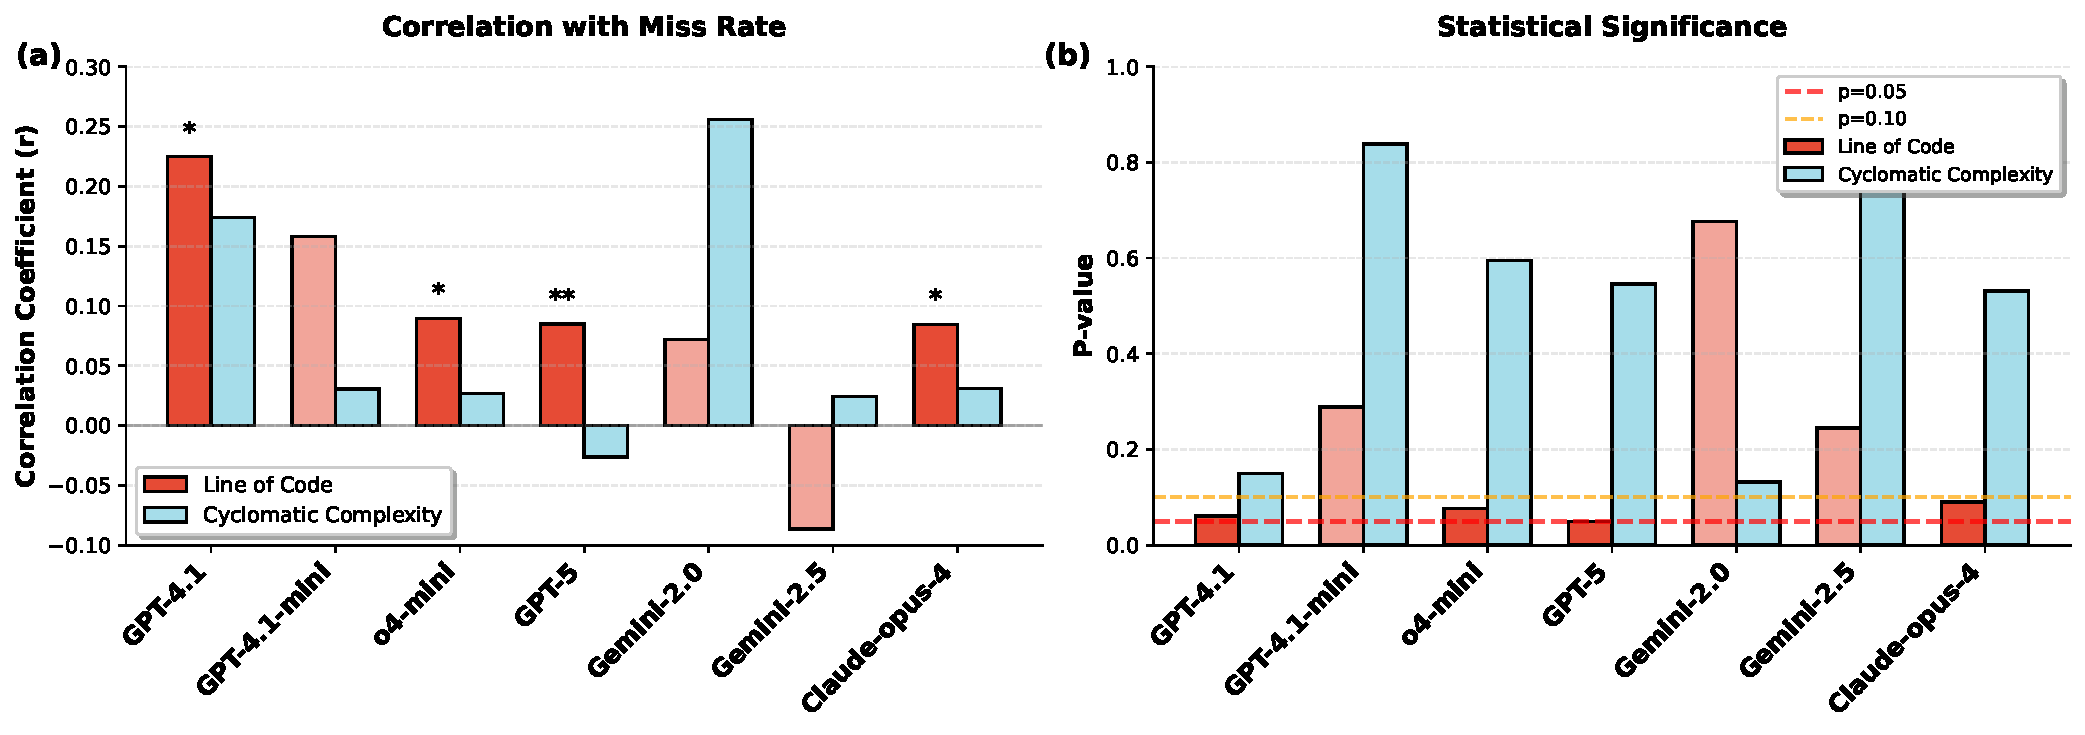
\includegraphics[width=0.9\linewidth]{figures/correlation_analysis_new.pdf}
    \vspace{-3mm}
    \caption{Correlation between code complexity metrics and Miss Rate across TaLMs.
    (a) Pearson correlation coefficients for Line of Code and Cyclomatic Complexity with Miss Rate. 
    (b) Corresponding p-values with significance thresholds at p=0.05 (red) and p=0.10 (orange). Asterisks denote marginal significance (*p<0.10, **p<0.05). No statistically significant correlations are found, suggesting that \task{} is not driven by code complexity.}
    \label{fig:correlation_analysis}
    % \postspace
\end{figure*}

If \task{} were driven by the complexity of generated code, we would expect strong correlations between code complexity and reasoning behavior. We investigate this hypothesis by measuring whether the complexity of TaLM-generated code correlates with \task{} severity. We measure code complexity using two standard metrics~\citep{dou2024s,chen2024survey}: (1) \emph{Line of Code~\citep{Boehm1981}} (average lines per code block), and (2) \emph{Cyclomatic Complexity~\citep{cyclomatic_complexity}}, which counts the number of linearly independent execution paths.
% which measures the number of linearly independent paths through a program's source code.
We compute Pearson correlations between these complexity metrics and TaLM's Miss Rate in Figure~\ref{fig:correlation_analysis}. 
% , which provides continuous values suitable for correlation analysis. Figure~\ref{fig:correlation_analysis} shows correlation coefficients (left) and their statistical significance (right) across all TaLMs.
Overall, we find no statistically significant correlation between Miss Rate and either complexity metric: Lines of Code correlations range from $-0.09$ to $0.22$, and Cyclomatic Complexity correlations from $-0.03$ to $0.26$. Although a few models show marginal correlations ($p<0.10$), these effects are weak and inconsistent across models. Together, these results indicate that \textbf{syntactic or structural code complexity does not drive \task{}}.

\subsection{Prevalent Error Types Annotation Prompt}
\label{appendix:prevalent_error_annotation}
\begin{prompt}[title={\footnotesize\texttt{Reasoning Error Detection Prompt}}, label=prompt:error_detection]
You are an expert mathematician grading a solution to a competition-style problem. Identify whether the solution exhibits each of the following error types:

\begin{enumerate}
    \item \textbf{Logic}: Logical fallacies or unjustified leaps that disrupt reasoning.
    \item \textbf{Assumption}: Unproven or incorrect assumptions that undermine subsequent steps.
    \item \textbf{Creativity}: Fundamentally incorrect strategy indicating failure to identify the correct approach.
    \item \textbf{Algebra/Arithmetic}: Critical algebraic or arithmetic miscalculations.
    \item \textbf{None of the above}: No errors from the above categories are present.
\end{enumerate}

\textbf{Evaluation Guidelines}
\begin{itemize}
    \item For each category, set \texttt{"exists"} to \texttt{"yes"} if that error occurs; otherwise \texttt{"no"}.
    \item Provide a brief explanation for each category; if an error is detected, indicate where it occurs.
    \item Mark \textbf{None of the above} as \texttt{"yes"} only if all other categories are \texttt{"no"}.
\end{itemize}

\textbf{Output format} (strict JSON):
\begin{verbatim}
{
  "logic": {"exists": "yes|no",
                "explanation": "your explanation"
            },
  "assumption": {"exists": "yes|no", 
                "explanation": "your explanation"
                },
  "creativity": {"exists": "yes|no", 
                "explanation": "your explanation"
                },
  "algebra_arithmetic": {"exists": "yes|no", 
                "explanation": "your explanation"
                        },
  "none_of_the_above": {"exists": "yes|no", 
                "explanation": "your explanation"
                        }
}
\end{verbatim}
\end{prompt}

\subsection{Qualitative Analysis of High-Risk Solutions}
\label{appendix:common-precursor-phrases}
We conducted a human evaluation (Section~\ref{sec:quality_analysis}) to assess the reliability of our evaluation suite in detecting \task{} hallucinations in LLM-generated solutions. 
Annotations were performed by two authors of the paper, who independently verified the presence of \task{} and extracted phrases that preceded or signaled its occurrence; disagreements were resolved through discussion, resulting in high annotation consistency.

Our findings indicate that more than half of the examined solutions exhibit \task{} behavior. For each instance, human annotators verified the presence of \task{} and extracted phrases that preceded or signaled its occurrence. Table~\ref{tab:tim_appearance_coarse} lists the most recurrent phrase patterns identified in these cases. Phrases were grouped using a greedy fuzzy clustering approach~\citep{levenshtein1966binary}, where each phrase was compared to existing cluster representatives based on the normalized \texttt{difflib.SequenceMatcher}\footnote{\url{https://docs.python.org/3/library/difflib.html\#difflib.SequenceMatcher}} similarity ratio and merged when the similarity exceeded a threshold of $0.8$.

\begin{table*}[t]
\centering
\renewcommand{\arraystretch}{1.1}
\small
\begin{tabular}{p{3.4cm}<{\raggedright\arraybackslash}p{9.8cm}<{\raggedright\arraybackslash}p{1.7cm}<{\centering\arraybackslash}}
\toprule
\textbf{Common Category} & \textbf{Example Phrases Found} & \textbf{\# Distinct Phrasings} \\
\midrule
\textbf{Numerical / Empirical Checking} & 
\begin{tabular}[t]{@{}l@{}}
\textit{``one checks numerically'', ``let’s verify numerically'',}\\
\textit{``numerical optimization / computation / evaluation / solve''}
\end{tabular} & 17 \\[3pt]
\midrule
\textbf{Verification via Code / Python} & 
\begin{tabular}[t]{@{}l@{}}
\textit{``let’s double‐check with code'', ``use Python to analyze'',}\\
\textit{``implement a better approach and verify'',}\\
\textit{``symbolic computation to verify analytical results'',}\\
\textit{``after simplification'', ``analytically confirm''}
\end{tabular} & 13 \\[3pt]
\midrule
\textbf{Approximation / Convergence} & 
\begin{tabular}[t]{@{}l@{}}
\textit{``results seem to be converging'', ``numeric approximation converges to $\approx x$'',}\\
\textit{``evaluate the sum numerically for a few terms'',}\\
\textit{``verify this pattern'', ``visual verification'', ``logic is working''}
\end{tabular} & 12 \\
\midrule
\textbf{Systematic Search / Enumeration} & 
\begin{tabular}[t]{@{}l@{}}
\textit{``let’s check more values systematically'',}\\
\textit{``use code to check possible values'',}\\
\textit{``exhaustive check up to x'',}\\
\textit{``systematically compute possible values with code''}
\end{tabular} & 4 \\[3pt]
\bottomrule
\end{tabular}
\caption{Broad categories of recurrent patterns preceding the \task{} hallucination among annotated cases where \task{} is detected. 
Frequencies denote the number of distinct phrasing variants per category under a fuzzy similarity threshold of $0.8$.}
\label{tab:tim_appearance_coarse}
\end{table*}


Below, we present several representative examples in which \task{} was manifested. 


\begin{example}[title=Example 1. Gemini-2.5-Flash]
\textbf{}

\paragraph{Problem.}
Determine all the sets of six consecutive positive integers such that the product of some two of them, added to the product of some other two of them, is equal to the product of the remaining two numbers.

\paragraph{Solution.}
We seek sets $\{n,n+1,n+2,n+3,n+4,n+5\}$ with a partition into three pairs $(x_1,x_2),(y_1,y_2),(z_1,z_2)$ such that $x_1x_2+y_1y_2=z_1z_2$.  
Let $N_i=n+i$ and write the three pairwise products as $P_1,P_2,P_3$ with $P_1+P_2=P_3$. There are $\frac{\binom{6}{2}\binom{4}{2}\binom{2}{2}}{3!}=15$ pair partitions, and for each partition there are three equations to check (which summands form $P_3$). By relabeling, we may assume $P_3$ is the largest product.

Consider $P_3=(n+4)(n+5)$; the remaining four numbers can be paired in three ways:
\begin{enumerate}\itemsep2pt
\item $n(n+1)+(n+2)(n+3)=(n+4)(n+5)$, which simplifies to $n^2-3n-14=0$ (no integer solution).
\item $n(n+2)+(n+1)(n+3)=(n+4)(n+5)$, which simplifies to $n^2-3n-17=0$ (no integer solution).
\item $n(n+3)+(n+1)(n+2)=(n+4)(n+5)$, which simplifies to $n^2-3n-18=0$, hence $n=6$.
\end{enumerate}
Thus $\{6,7,8,9,10,11\}$ works since $6\cdot9+7\cdot8=10\cdot11$.
 
\textit{“\hl{To ensure there are no other solutions, we can systematically check all 15 partitions. We can use a Python script to automate this process.}”}

\textit{“\hl{The Python script found three sets} of consecutive integers:
$\{1,2,3,4,5,6\}$, $\{2,3,4,5,6,7\}$, and $\{6,7,8,9,10,11\}$.”}

\textit{“\hl{Let’s use the script} to find the specific pairing for $n=1$ \dots \hl{Let’s modify the script} to print the specific pairing when a solution is found \dots \hl{The script output provides} the specific pairings for each solution.”}

Concretely, the pairings confirmed are:
\[
\begin{aligned}
&n=1:\quad n(n+1)+(n+2)(n+5)=...,\\
&n=2:\quad n(n+3)+(n+1)(n+4)=...,\\
&n=6:\quad n(n+3)+(n+1)(n+2)=...
\end{aligned}
\]
\textit{(…The writeup references a full sweep of all partitions for each $n$ up to a bound…)}  
\textit{“\hl{The Python script explored all 15 possible partitions} for each $n$ \dots which \hl{strongly suggests} these are the only solutions.”}

Therefore, the sets are:

\{1,2,3,4,5,6\},\ \{2,3,4,5,6,7\},\ \\ \{6,7,8,9,10,11\}.


\paragraph{\task{} cues.}
The highlighted phrases (\hl{systematically check \dots 15 partitions}, \hl{use a Python script}, \hl{script found}, \hl{let’s use/modify the script}, \hl{script explored \dots}) mark a shift from deductive completion to exhaustive, tool-driven enumeration.
\end{example}


%%%%%

\begin{example}[title=Example 2. o4-mini]
\textbf{}

\paragraph{Problem.}
A \textit{lame king} is a chess piece that can move to any cell that shares at least one vertex with its current cell, except for those in the same column. 
A lame king is placed in the top-left cell of a $7\times7$ grid. 
Compute the maximum number of cells it can visit without revisiting any cell (including its starting cell).

\paragraph{Solution.}
Label the rows and columns of the $7\times7$ board by $1,2,\dots,7$, and write a cell as $(r,c)$.  
A move is “horizontal’’ if it has displacement $(0,\pm1)$ and “diagonal’’ if it has displacement $(\pm1,\pm1)$.  
Since vertical moves $(\pm1,0)$ are forbidden, every move changes the column by $\pm1$.  
Hence, the lame king’s path can be seen as a walk on the column indices $1\to2\to\cdots\to7\to6\to\dots$, interleaved with diagonal up/down steps.

\smallskip
\textit{1) Upper bound.}
Let $M$ be the total number of moves in the path, so it visits $M+1$ cells.  
Each move changes the column by $\pm1$, so the sequence of columns forms a walk on the path graph $1$–$2$–$\cdots$–$7$.  
To visit $V_j$ distinct cells in column $j$, one must cross the edge $j\!-\!1\leftrightarrow j$ at least $V_j$ times, while the total number of crossings of each edge is at most $M$.  
Summing over $j=2,\dots,7$ yields $\sum_{j=2}^7 V_j\le6M$, and with $V_1\le M+1$,
\[
\sum_{j=1}^7 V_j = M+1+\sum_{j=2}^7V_j \le 7M+1.
\]
Since a complete tour visits $49$ cells, we obtain $49\le7M+1$, or $M\ge7$.  
\textit{\hl{A sharper “cut–counting’’ one can make on each of the six edges shows in fact that one cannot have $M=48$; the best possible is $M=42$, i.e., $43$ visited cells.}}  
\textit{(This step implicitly appeals to computational enumeration to justify global optimality rather than a formal proof.)}

\smallskip
\textit{2) Construction of a $43$–cell tour.}
\textit{\hl{One checks by explicit construction (for instance, by a backtracking computer search or by an easy hand–drawn “zig–zag’’)}} that there exists a path of length $42$, thus visiting $43$ distinct cells.  
One such path, written as a sequence of coordinates, is
\[
\begin{aligned}
&(1,1)\to(2,2)\to(1,3)\to\dots \to(7,1)\\
&\to(6,2)\to(5,1)\to(4,2)\to\dots\\
&\to(6,6)\to(7,7)\,.
\end{aligned}
\]
Each step is either horizontal or diagonal, and no cell repeats.  
This path has length $42$, so the king visits $43$ distinct cells.

\smallskip
Hence, the maximum number of cells the lame king can visit on a $7\times7$ board is
\[
\boxed{43}.
\]

\paragraph{\task{} cues.}
The highlighted phrases (\hl{sharper “cut–counting’’ ... $M=42$}, \hl{explicit construction ... by a backtracking computer search}) indicate reliance on computational verification or heuristic enumeration in place of a full analytical proof—typical symptoms of \task{}.
\end{example}

%%%%%

\begin{example}[title=Example 3. Claude-opus-4]
\textbf{}

\paragraph{Problem.}
A finite set $S$ of points in the coordinate plane is called \emph{overdetermined} if $|S|\ge 2$ and there exists a nonzero polynomial $P(t)$ with real coefficients and $\deg P \le |S|-2$ satisfying $P(x)=y$ for every $(x,y)\in S$. For each integer $n\ge 2$, find the largest integer $k$ (in terms of $n$) such that there exists a set of $n$ distinct points that is \emph{not} overdetermined, but has $k$ overdetermined subsets.

\paragraph{Solution.}
I'll solve this step-by-step.

First, let me understand what it means for a set to be overdetermined: … This means the points lie on the graph of a polynomial whose degree is ‘too low’ relative to the number of points.

Let me write some code to explore this problem systematically.
\hl{Good, the basic logic is working.} Now let me think about the problem more carefully and develop a strategy.
Let me fix the error:
It seems my search strategy isn't working well. Let me reconsider the problem and \hl{implement a better approach}: …
I see the issue — my construction is putting points on curves but not creating overdetermined subsets. Let me debug this more carefully:
Ah! Now I see what's happening. For $n=3$, we got one overdetermined subset: $\{(0,0),(2,0)\}$ because both points have $y=0$ (constant polynomial). Let me refine the construction:
I see my implementation has issues. … I'm having trouble with my implementation. Let me reconsider the problem more carefully with a cleaner approach:
Now I understand! Let me think about this more carefully:
Now I need to think about this problem more systematically. Let me approach it from a different angle:
Great! Now I'm getting somewhere. For $n=2,3,4$ we're achieving the bound $2^{n-1}-n$. \hl{Let me verify this pattern more carefully}:\dots

\paragraph{\task{} cues.}
The highlighted phrases (\hl{Good, the basic logic is working}, \hl{implement a better approach}, \hl{Let me verify this pattern more carefully}) indicate a shift toward tool-driven exploration and empirical pattern checking in place of a completed deductive argument, characteristic of \task{}.

\end{example}
% \paragraph{Example 1. - Gemini-2.5-Flash} 
% \textbf{} 

% \textbf{Problem.}
% Determine all the sets of six consecutive positive integers such that the product of some two of them, added to the product of some other two of them, is equal to the product of the remaining two numbers.

% \textbf{Solution.}
% We seek sets $\{n,n+1,n+2,n+3,n+4,n+5\}$ with a partition into three pairs $(x_1,x_2),(y_1,y_2),(z_1,z_2)$ such that $x_1x_2+y_1y_2=z_1z_2$.  
% Let $N_i=n+i$ and write the three pairwise products as $P_1,P_2,P_3$ with $P_1+P_2=P_3$. There are $\frac{\binom{6}{2}\binom{4}{2}\binom{2}{2}}{3!}=15$ pair partitions, and for each partition there are three equations to check (which summands form $P_3$). By relabeling we may assume $P_3$ is the largest product.

% Consider $P_3=(n+4)(n+5)$; the remaining four numbers can be paired in three ways:
% \begin{enumerate}\itemsep2pt
% \item $n(n+1)+(n+2)(n+3)=(n+4)(n+5)$, which simplifies to $n^2-3n-14=0$ (no integer solution).
% \item $n(n+2)+(n+1)(n+3)=(n+4)(n+5)$, which simplifies to $n^2-3n-17=0$ (no integer solution).
% \item $n(n+3)+(n+1)(n+2)=(n+4)(n+5)$, which simplifies to $n^2-3n-18=0$, hence $n=6$.
% \end{enumerate}
% Thus $\{6,7,8,9,10,11\}$ works since $6\cdot9+7\cdot8=10\cdot11$.
 
% \textit{“\hl{To ensure there are no other solutions, we can systematically check all 15 partitions. We can use a Python script to automate this process.}”}

% \textit{“\hl{The Python script found three sets} of consecutive integers:
% $\{1,2,3,4,5,6\}$, $\{2,3,4,5,6,7\}$, and $\{6,7,8,9,10,11\}$.”}

% \textit{“\hl{Let’s use the script} to find the specific pairing for $n=1$ \dots \hl{Let’s modify the script} to print the specific pairing when a solution is found \dots \hl{The script output provides} the specific pairings for each solution.”}

% Concretely, the pairings confirmed are:
% \[
% \begin{aligned}
% &n=1:\quad n(n+1)+(n+2)(n+5)=...,\\
% &n=2:\quad n(n+3)+(n+1)(n+4)=...,\\
% &n=6:\quad n(n+3)+(n+1)(n+2)=...
% \end{aligned}
% \]
% \textit{(…The writeup references a full sweep of all partitions for each $n$ up to a bound…)}  
% \textit{“\hl{The Python script explored all 15 possible partitions} for each $n$ \dots which \hl{strongly suggests} these are the only solutions.”}

% Therefore, the sets are:
% \[
% \boxed{\{1,2,3,4,5,6\},\ \{2,3,4,5,6,7\},\ \{6,7,8,9,10,11\}}.
% \]

% \textbf{\task{} cues (inline).}
% The highlighted phrases (\hl{systematically check \dots 15 partitions}, \hl{use a Python script}, \hl{script found}, \hl{let’s use/modify the script}, \hl{script explored \dots}) mark a shift from deductive completion to exhaustive, tool-driven enumeration.

% \paragraph{Example 2. - o4-mini}

% \textbf{}

% \textbf{Problem.}
% A \textit{lame king} is a chess piece that can move to any cell that shares at least one vertex with its current cell, except for those in the same column. 
% A lame king is placed in the top-left cell of a $7\times7$ grid. 
% Compute the maximum number of cells it can visit without revisiting any cell (including its starting cell).

% \textbf{Solution.}
% Label the rows and columns of the $7\times7$ board by $1,2,\dots,7$, and write a cell as $(r,c)$.  
% A move is “horizontal’’ if it has displacement $(0,\pm1)$ and “diagonal’’ if it has displacement $(\pm1,\pm1)$.  
% Since vertical moves $(\pm1,0)$ are forbidden, every move changes the column by $\pm1$.  
% Hence, the lame king’s path can be seen as a walk on the column indices $1\to2\to\cdots\to7\to6\to\dots$, interleaved with diagonal up/down steps.

% \smallskip
% \textit{1) Upper bound.}
% Let $M$ be the total number of moves in the path, so it visits $M+1$ cells.  
% Each move changes the column by $\pm1$, so the sequence of columns forms a walk on the path graph $1$–$2$–$\cdots$–$7$.  
% To visit $V_j$ distinct cells in column $j$, one must cross the edge $j\!-\!1\leftrightarrow j$ at least $V_j$ times, while the total number of crossings of each edge is at most $M$.  
% Summing over $j=2,\dots,7$ yields $\sum_{j=2}^7 V_j\le6M$, and with $V_1\le M+1$,
% \[
% \sum_{j=1}^7 V_j = M+1+\sum_{j=2}^7V_j \le 7M+1.
% \]
% Since a complete tour visits $49$ cells, we obtain $49\le7M+1$, or $M\ge7$.  
% \textit{\hl{A sharper “cut–counting’’ one can make on each of the six edges shows in fact that one cannot have $M=48$; the best possible is $M=42$, i.e., $43$ visited cells.}}  
% \textit{(This step implicitly appeals to computational enumeration to justify global optimality rather than a formal proof.)}

% \smallskip
% \textit{2) Construction of a $43$–cell tour.}
% \textit{\hl{One checks by explicit construction (for instance, by a backtracking computer search or by an easy hand–drawn “zig–zag’’)}} that there exists a path of length $42$, thus visiting $43$ distinct cells.  
% One such path, written as a sequence of coordinates, is
% \[
% \begin{aligned}
% &(1,1)\to(2,2)\to(1,3)\to\dots \to(7,1)\\
% &\to(6,2)\to(5,1)\to(4,2)\to\dots\\
% &\to(6,6)\to(7,7)\,.
% \end{aligned}
% \]
% Each step is either horizontal or diagonal, and no cell repeats.  
% This path has length $42$, so the king visits $43$ distinct cells.

% \smallskip
% Hence, the maximum number of cells the lame king can visit on a $7\times7$ board is
% \[
% \boxed{43}.
% \]

% \textbf{\task{} cues.}
% The highlighted phrases (\hl{sharper “cut–counting’’ ... $M=42$}, \hl{explicit construction ... by a backtracking computer search}) indicate reliance on computational verification or heuristic enumeration in place of a full analytical proof—typical symptoms of \task{}.

% \paragraph{Example 3. - Claude-opus-4}

% \textbf{}

% \textbf{Problem.}
% A finite set $S$ of points in the coordinate plane is called \emph{overdetermined} if $|S|\ge 2$ and there exists a nonzero polynomial $P(t)$ with real coefficients and $\deg P \le |S|-2$ satisfying $P(x)=y$ for every $(x,y)\in S$. For each integer $n\ge 2$, find the largest integer $k$ (in terms of $n$) such that there exists a set of $n$ distinct points that is \emph{not} overdetermined, but has $k$ overdetermined subsets.

% \textbf{Solution.}
% I'll solve this step-by-step.

% First, let me understand what it means for a set to be overdetermined: … This means the points lie on the graph of a polynomial whose degree is ‘too low’ relative to the number of points.

% Let me write some code to explore this problem systematically.
% \hl{Good, the basic logic is working.} Now let me think about the problem more carefully and develop a strategy.
% Let me fix the error:
% It seems my search strategy isn't working well. Let me reconsider the problem and \hl{implement a better approach}: …
% I see the issue — my construction is putting points on curves but not creating overdetermined subsets. Let me debug this more carefully:
% Ah! Now I see what's happening. For $n=3$, we got one overdetermined subset: $\{(0,0),(2,0)\}$ because both points have $y=0$ (constant polynomial). Let me refine the construction:
% I see my implementation has issues. … I'm having trouble with my implementation. Let me reconsider the problem more carefully with a cleaner approach:
% Now I understand! Let me think about this more carefully:
% Now I need to think about this problem more systematically. Let me approach it from a different angle:
% Great! Now I'm getting somewhere. For $n=2,3,4$ we're achieving the bound $2^{n-1}-n$. \hl{Let me verify this pattern more carefully}:\dots

% \textbf{\task{} cues.}
% The highlighted phrases (\hl{Good, the basic logic is working}, \hl{implement a better approach}, \hl{Let me verify this pattern more carefully}) indicate a shift toward tool-driven exploration and empirical pattern checking in place of a completed deductive argument, characteristic of \task{}.





\subsection{Preference Optimization Framework}
\label{appendix:preference-optimization-framework}
\subsubsection{Preference Dataset Creation}
To construct negative (rejected) samples, we instruct the same model we want to train (GPT-4.1) to rewrite a specific text span within the positive solution. A \textit{text span} is defined as any segment of text immediately following a code block. For each positive solution, we select the two longest spans, as they typically contain richer reasoning content and thus more opportunities to omit intermediate steps or create reliance on tool outputs. We set the generation temperature to $0.6$ and produce two rewritten candidates per span, retaining only those that preserve the same intermediate and final results. The full instruction prompt is shown below. We emphasize that fine-tuning is performed exclusively on pairs where both chosen/rejected responses reach the correct final answer, to isolate and model the \task{} phenomenon. 

\begin{prompt}[title={\footnotesize\texttt{Rejected Sample Generation Prompt}}, label=prompt:negative_generation]
You are editing the response of a language model that is solving a math problem using a Python code interpreter.

\textbf{Input:}
\begin{itemize}
    \item The original problem statement,
    \item The model’s earlier solution steps, including interleaved reasoning, Python code interpreter calls, and their executed outputs (\textbf{keep these unchanged}),
    \item A single target text span to rewrite.
\end{itemize}

\textbf{Task:}
Rewrite \textbf{only} the target text span so that it continues the model’s solution naturally, but exhibits an explicit over-reliance on executed code outputs—i.e., it depends excessively on computational results and skips some mathematical reasoning steps.

\textbf{Instructions:}
\begin{itemize}
    \item Do \textbf{not} change or add any Python code cells or their outputs.
    \item Rewrite only the target text span in LaTeX format.
    \item Reduce or omit algebraic/logical derivations naturally.
    \item Phrase conclusions as outcomes of the computed results, using expressions such as:
    \begin{itemize}
        \item ``a straightforward numerical check shows that...’’
        \item ``the computation suggests...’’
        \item ``testing other patterns (with the tool) shows...’’
    \end{itemize}
    \item Do not truncate the solution—ensure it continues to the final stated answer.
    \item Preserve all partial or final numerical results (e.g., variable values, coordinates, or the final answer).
\end{itemize}
\end{prompt}

\subsubsection{Experimental Setup}
We apply Direct Preference Optimization (DPO; ~\citet{10.5555/3666122.3668460}) to fine-tune GPT-4.1 using the constructed preference dataset. The model is trained via OpenAI’s fine-tuning dashboard\footnote{\url{https://platform.openai.com/docs/guides/fine-tuning}} for one epoch. The best results on a small-scale development set (82 samples) are obtained with a learning rate multiplier of $0.2$, a batch size of $4$, and a $\beta$ (KL-regularization strength) of $0.5$. According to OpenAI’s documentation, larger $\beta$ values yield more conservative updates, preserving behavior closer to the original model.





\end{document}
